\label{cha:sle}
As a practical application of the LaRCH model, the model is trained on a real single-cell RNA-seq dataset used to study the cell-type specific molecular and genetic associations of SLE \cite{sledata}. In this section, details of the scRNA-seq data are described and the resulting model trained on the dataset is used to explore various aspects of the disease pathogenesis of SLE.

\section{Single-cell RNA-seq data from a large SLE dataset}

The scRNA-seq dataset used to train the model is from a 2022 paper from Perez \textit{et al}. \cite{sledata}. This dataset consists of single-cell transcriptome data of 1.2 million PBMCS from 99 healthy control individuals and 162 individuals with SLE. 

\subsection{Dataset Details}

PBMC samples used in this analysis were collection from SLE cases in the California Lupus Epidemiological Study (CLUES) cohort. Matched healthy control samples were collected from the UCSF Rheumatology Clinic and the Immune Variaton Project (ImmVar) \cite{sledata}.

Single-cell gene expression profiles from pooled antibody-stained and unstained PBMCs was generated using 10x Genomics' Chromium Single Cell 3' V2 chemistry and processed with the 10x Cell Ranger pipeline. Filtered scRNA-seq read count data was obtained directly from accession number \href{https://www.ncbi.nlm.nih.gov/geo/query/acc.cgi}{GSE174188} in the Gene Expression Omnibus (GEO). Additionally, patient metadata, cell type annotation, and UMAP projections from the original study were used for the data analysis in this chapter.

\newpage 
\section{Deconvolution of Immune Cell Subtypes}

\begin{figure}
    \centering
    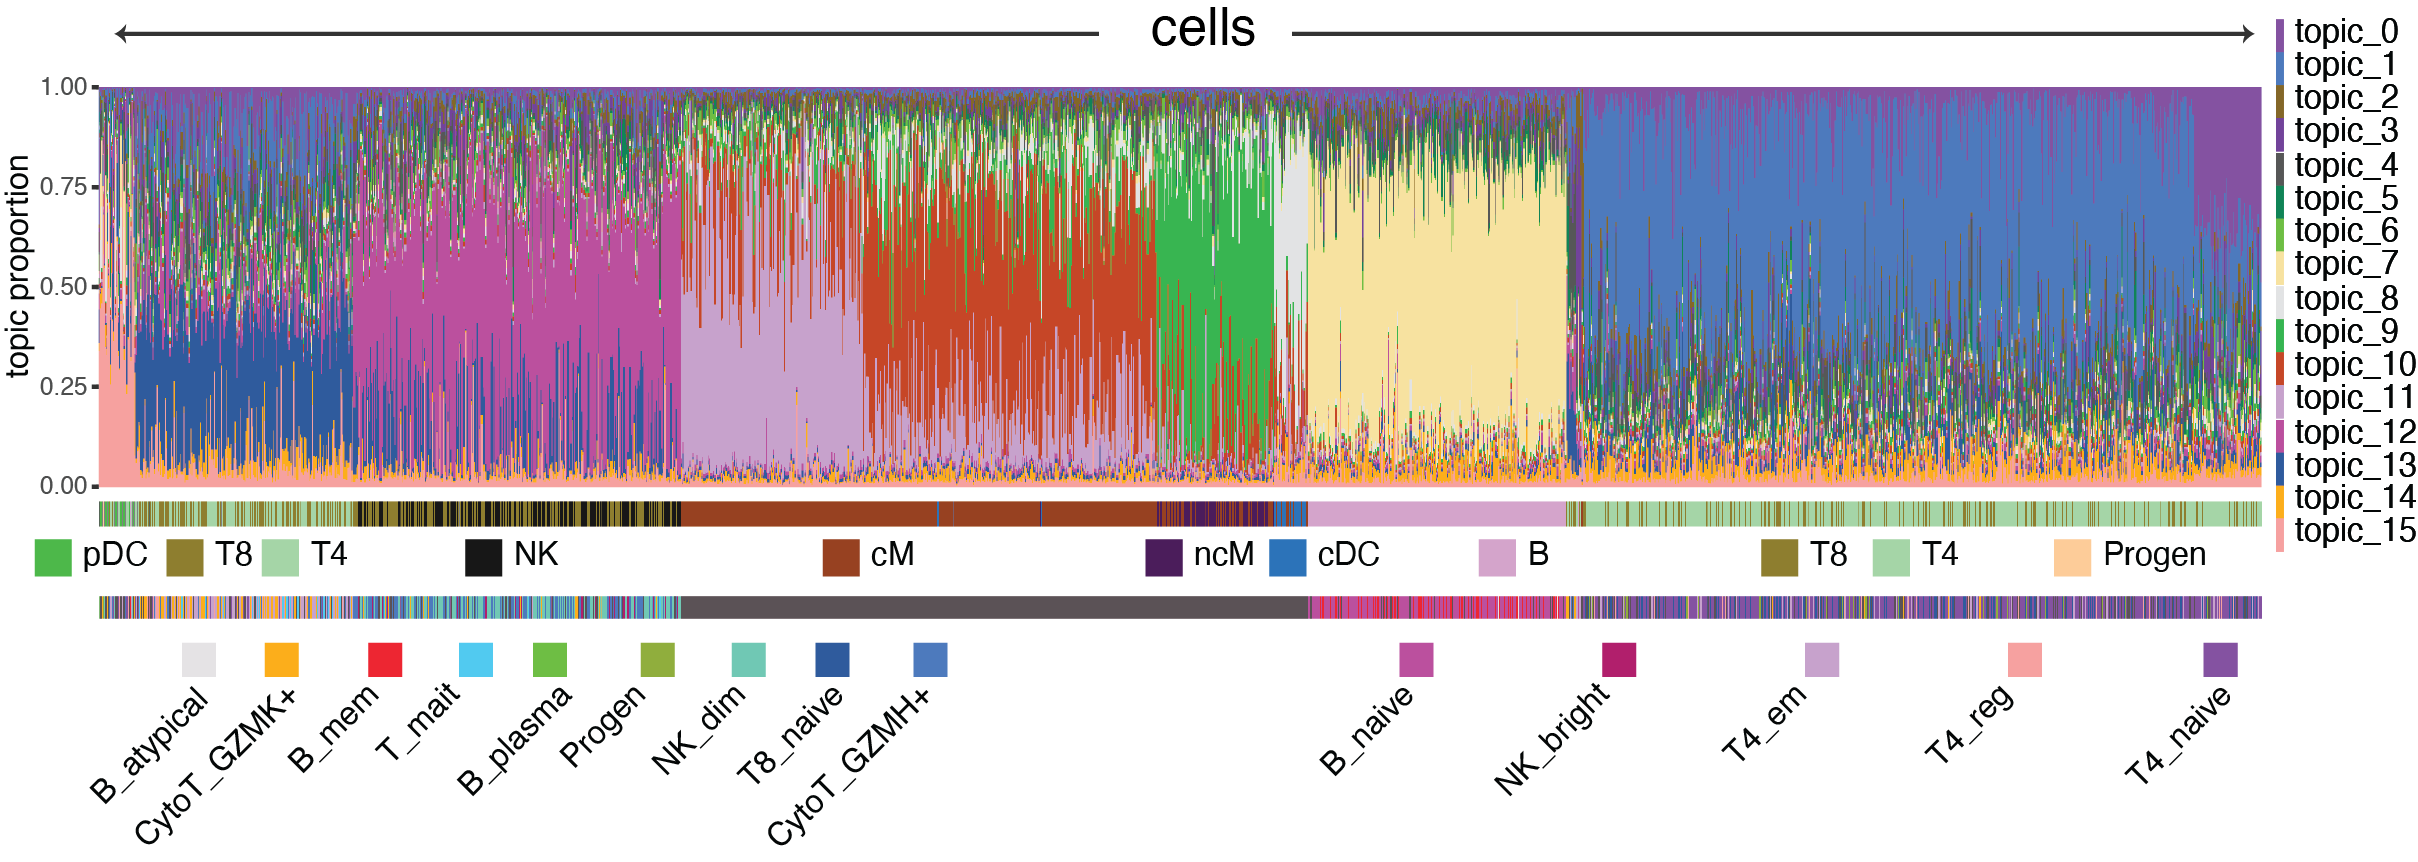
\includegraphics[width=\textwidth]{Figures/struct_plt.png}
    \caption{\textbf{Distinct topic proportions of PBMCs in a scRNA-seq dataset of SLE and healthy individuals correspond to cell type labels} Structure plot of estimated $\theta$ values for a subsample of 10,000 cells in the data set. Cells are annotated below by labelled cell types obtained from Perez \textit{et al.} \cite{sledata}}
    \label{fig:sle_struct}
\end{figure}

Estimated topic proportion profiles show distinct groups of cells within the latent space that align closely with the cell types determined in the original Perez \textit{et al.} paper \cite{sledata} (Fig.\ref{fig:sle_struct}). The topic representation of cells is able to pick up more granularity that potentially describes further distinct cell types, namely in the cells labelled as 'classical monocytes' where there are two distinct groups in the topic space primarily represented by either topic 10 or topic 11, suggesting classical monocyte-labeled subsets could be composed of subsets with differing cell function. 

\begin{figure}
    \centering
    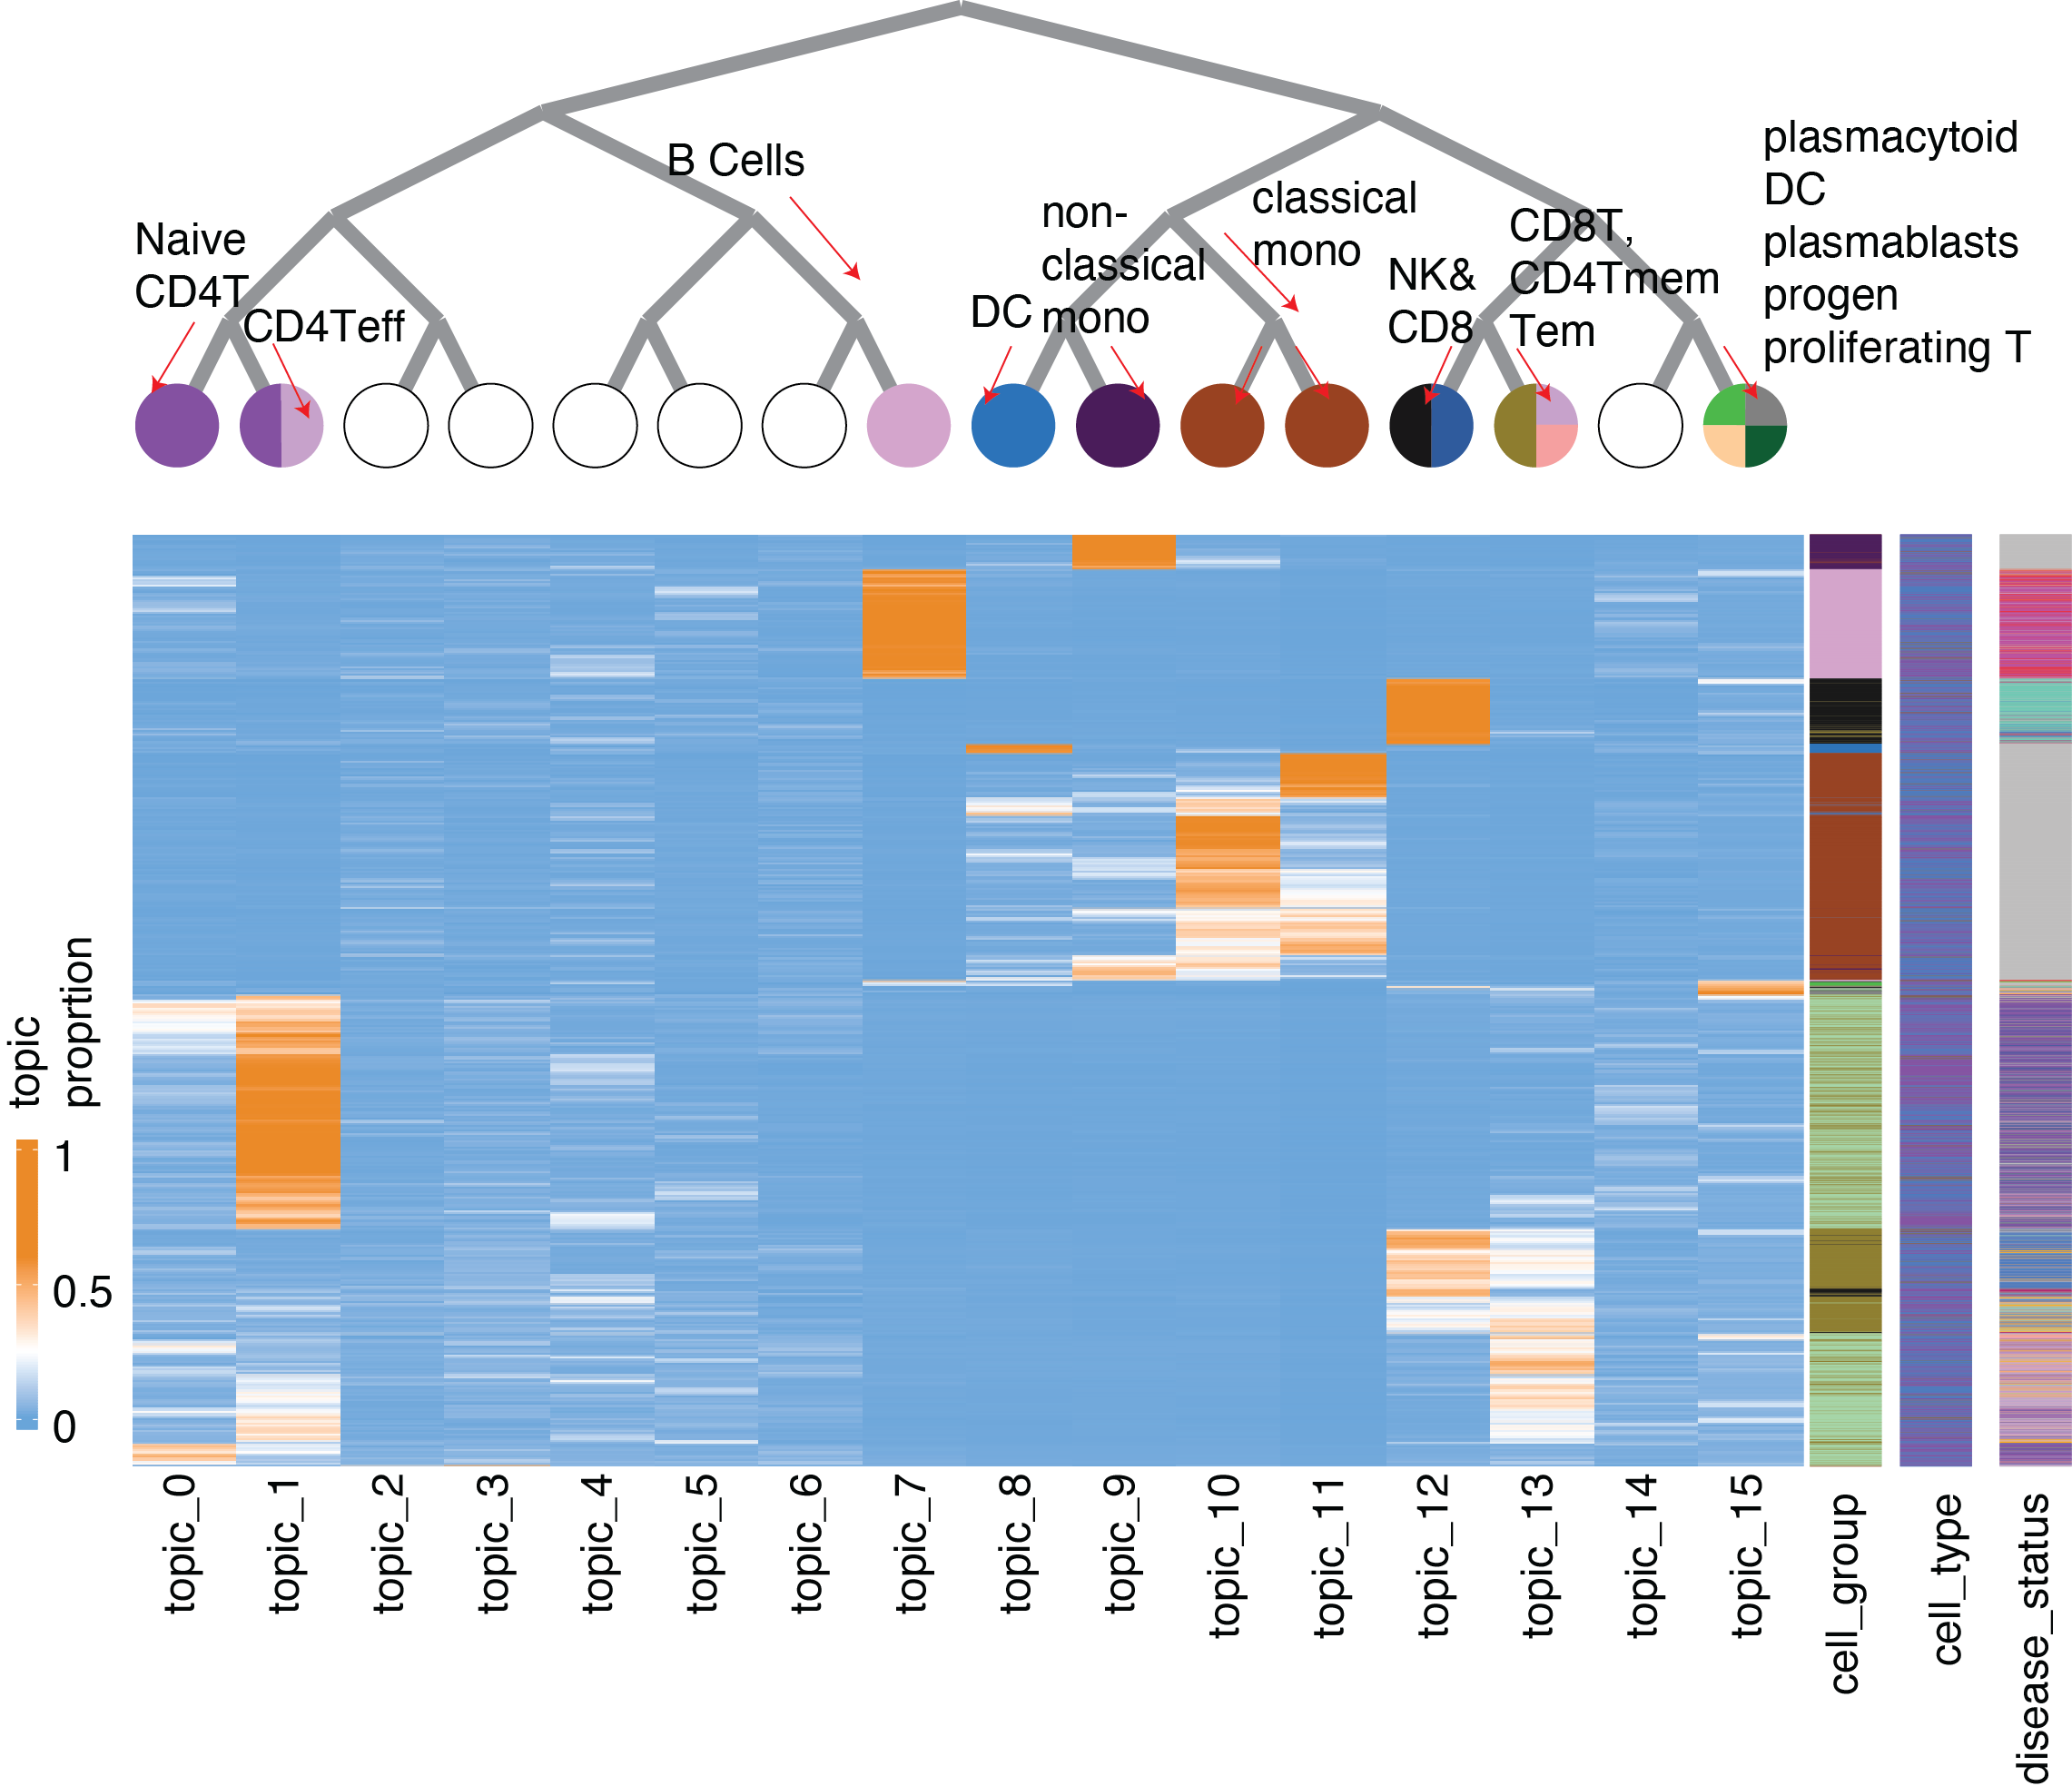
\includegraphics[width=\textwidth]{Figures/hier_tree.png}
    \caption{\textbf{Tree-structure relationships between cell types are reconstructed using latent topic profiles of a real scRNA-seq dataset} The top panel shows the reconstructed tree structure based on average latent topic profile representations of cell types. Below is a heatmap of the latent topic proportion profiles across a subset of 10,000 cells from the dataset.}
    \label{fig:sle_tree}
\end{figure}

As with the simulated data, a tree structure outlining the hierarchical relationships between cell types is qualitatively assembled using the average latent profiles of immune cell subsets. Similar to the simulated data setting, the constructed tree structure from the real data set aligns with the canonical understanding of immune cell differentiation (Fig.\ref{fig:sle_tree}). B cells lie within their own distinct branch of the tree. Myeloid cells, including monocytes and dendritic cells are contained within the tree branch with topics 8 through 11. Topic 15 captures a number of intermediate immune cell-states, including progenitor and proliferating lymphoid cells, proliferating dendritic cells, and plasmablasts. Naive CD4+ T cells are primarily represented by topic 0 and 1, while the remaining CD4+ subtypes are represented by topic 13 along with non-naive CD8+ T cells. NK cells and naive CD8+ T cells are found in topic 12. 

\subsection{Cell Clustering}
\begin{figure}
    \centering
    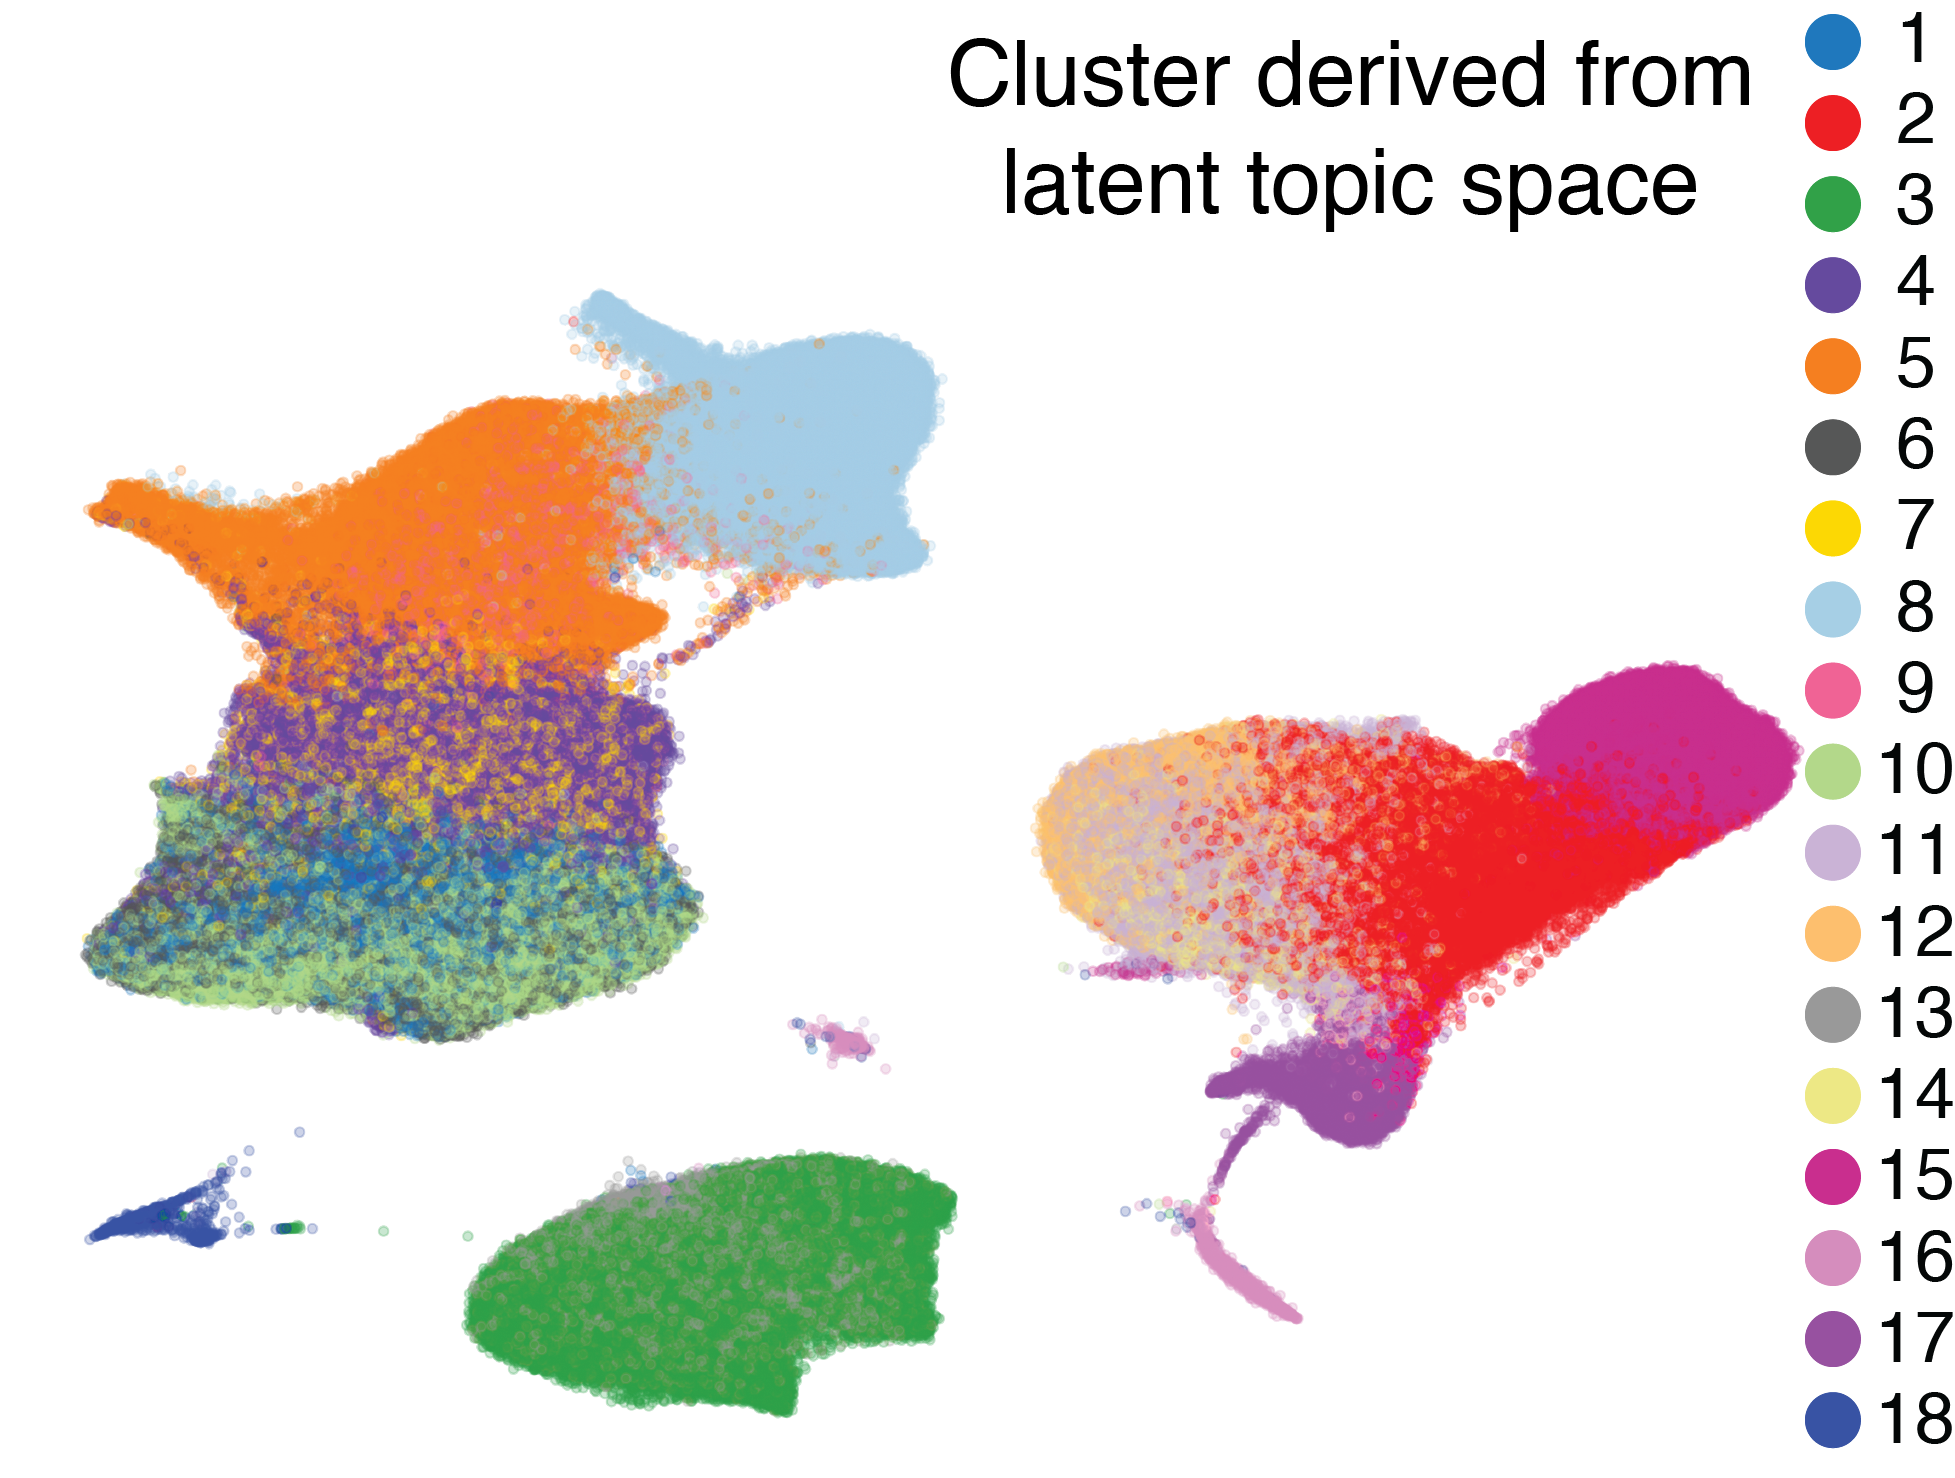
\includegraphics[width=\textwidth]{Figures/cluster_umap.png}
    \caption{\textbf{Clustering on latent topic space recovers groups of immune cells belonging to related immune subsets} UMAP projection of scRNA-seq data are coloured by Louvain clusters derived from the latent topic space. UMAP projection values obtained from the original Perez \textit{et al.} study \cite{sledata}}
    \label{fig:cluster_umap}
\end{figure}

\begin{figure}
    \centering
    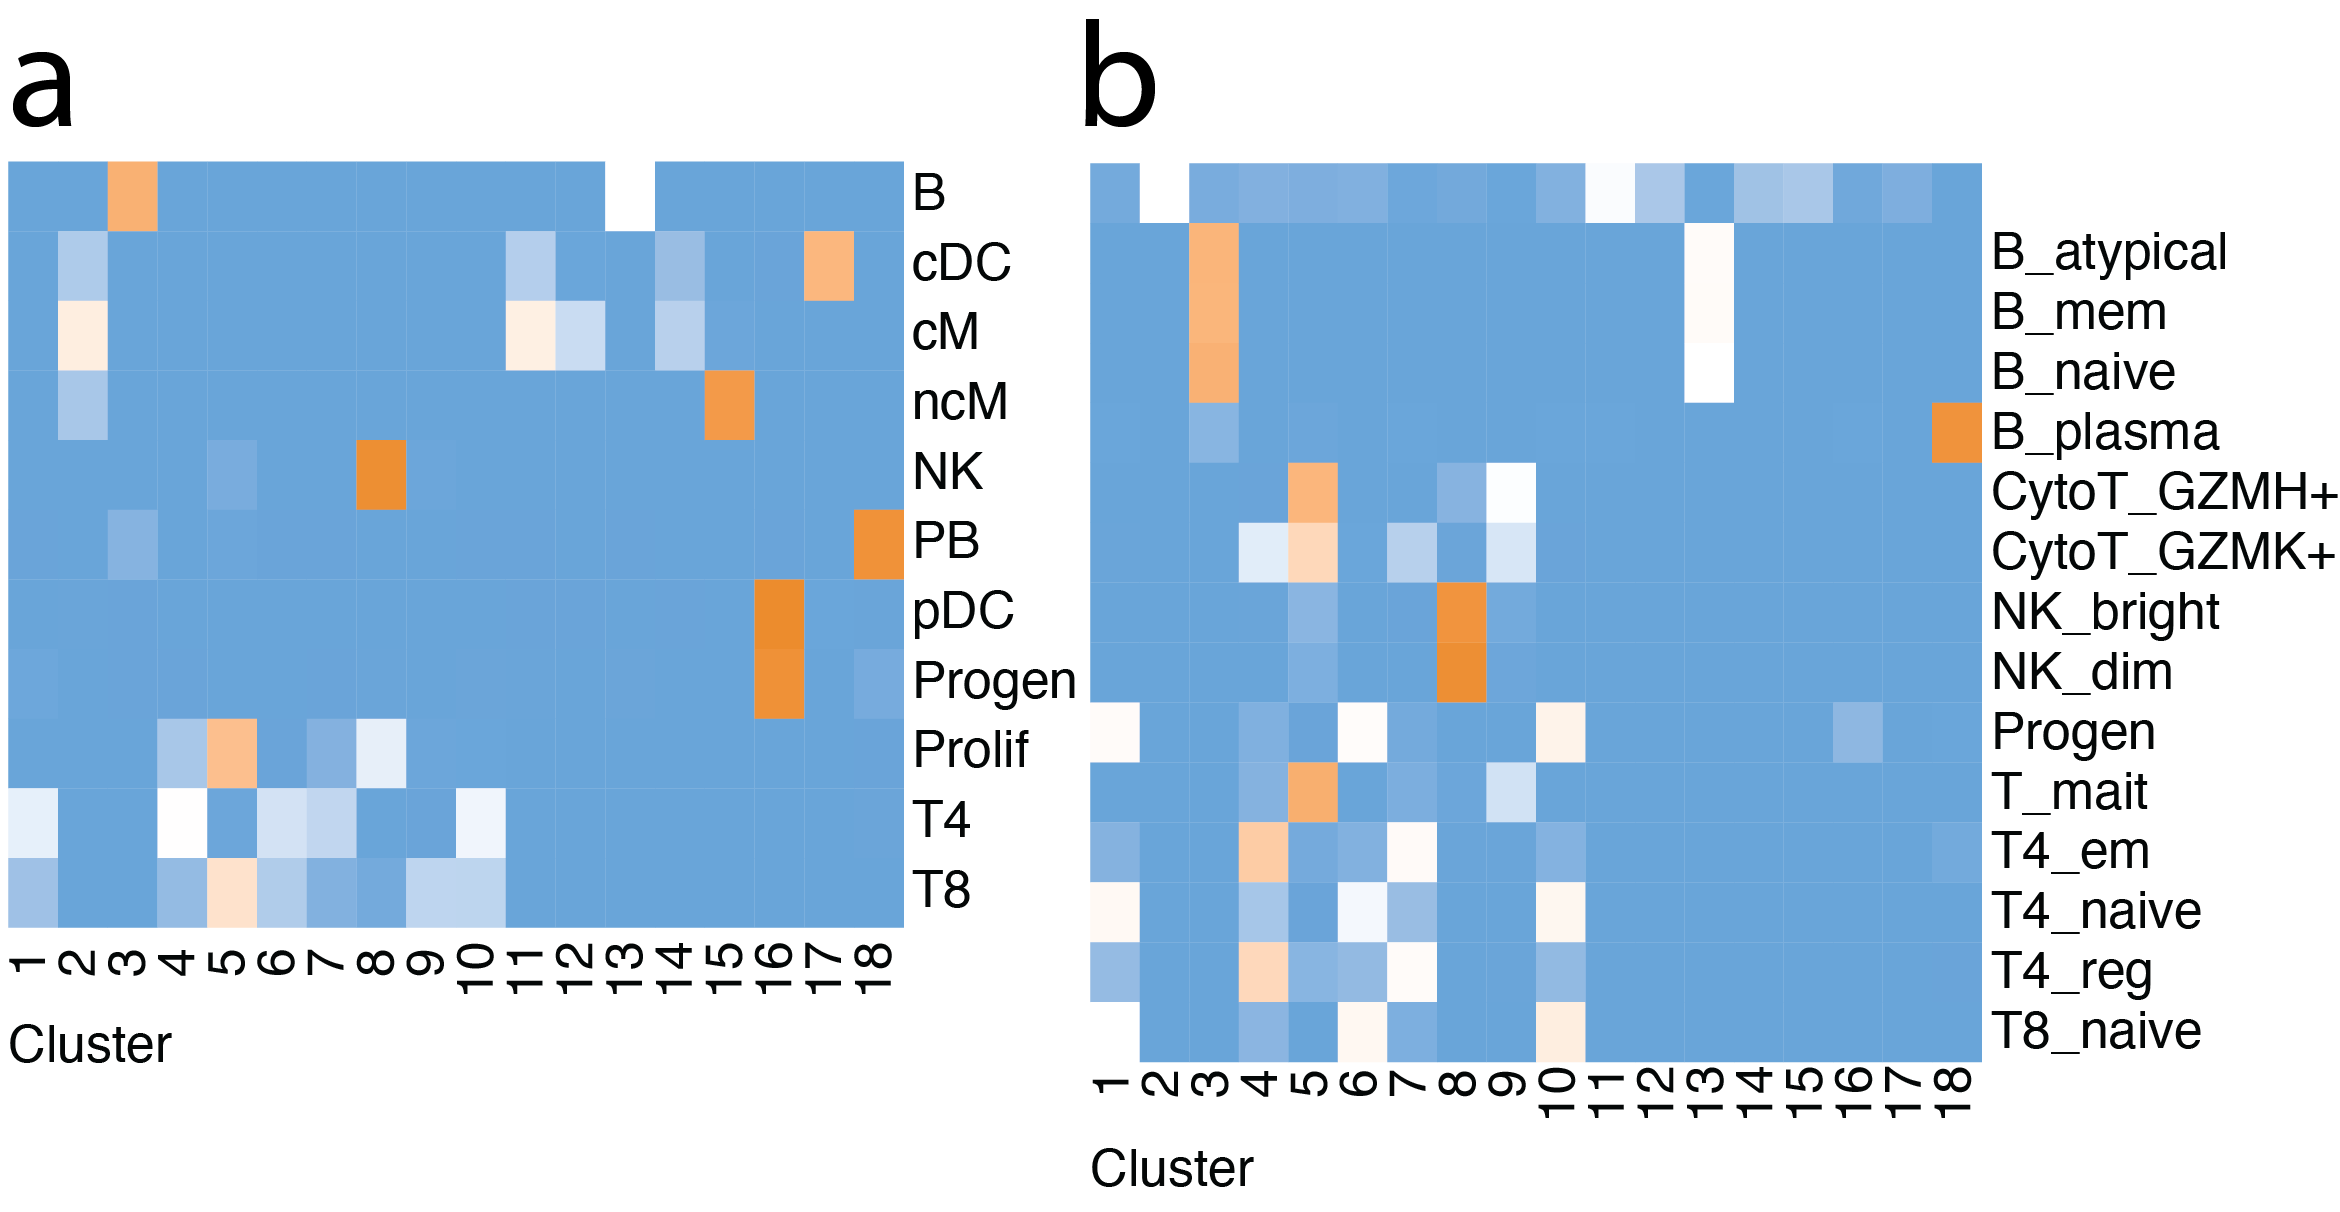
\includegraphics[width=\textwidth]{Figures/cluster_ct.png}
    \caption{\textbf{Overlap exists between latent topic clusters and original cell labels} a) Heatmap depicting the similarity matrix between louvain clusters obtained from latent topic space and cell group labels. b) Heatmap depicting  the similarity matrix between louvain clusters obtained from latent topic space and cell type labels. 
    Cell clusters are represented along the columns of the heatmap while cell labels are represented along the rows. 
    Cell group and cell types are described in \cite{sledata}. Cell groups describe more general immune cell subsets while cell types describe specific immune cell subsets.}
    \label{fig:cluster_ct}
\end{figure}

Louvain clustering \cite{louvain} using $k=30$ nearest neighbours in the latent topic space results in clustering that aligns with cell groups described by Perez \textit{et al.} \cite{sledata} (Fig.\ref{fig:cluster_umap}, \ref{fig:cluster_ct}a), but quickly loses the ability to clearly distinguish cell the more specific cell types (Fig.\ref{fig:cluster_ct}b). For this purpose, similarity is measured as the proportion of cells with a specified label contained within a cluster, mathematically this is: 
\begin{align*}
    &\text{Similarity}(\text{cell\_label}_j, \text{cluster}_k) = \\ &\frac{\sum_{i = 0}^N \mathbb{I}(\text{cell\_label}(\text{cell}_i) = \text{cell\_label}_j) * \mathbb{I}(\text{cluster}(\text{cell}_i) = \text{cluster}_k)}{\sum_{i = 0}^N \mathbb{I}(\text{cell\_label}(\text{cell}_i) = \text{cell\_label}_j)}
\end{align*} 
Where $N$ is total number of cells in the dataset and cell\_label(cell$_i$) and cluster(cell$_i$) return the assigned cell label and cluster for cell$_i$, respectively.

Since the original cell types are assigned from Louvain clustering on UMAP reduced dimensions and canonical marker gene expression, it is unclear as to which clustering method produces higher-quality immune function-relevant cluster assignments. 

\newpage
\section{Disease Dependent Differences in Expression}

\begin{figure}
    \centering
    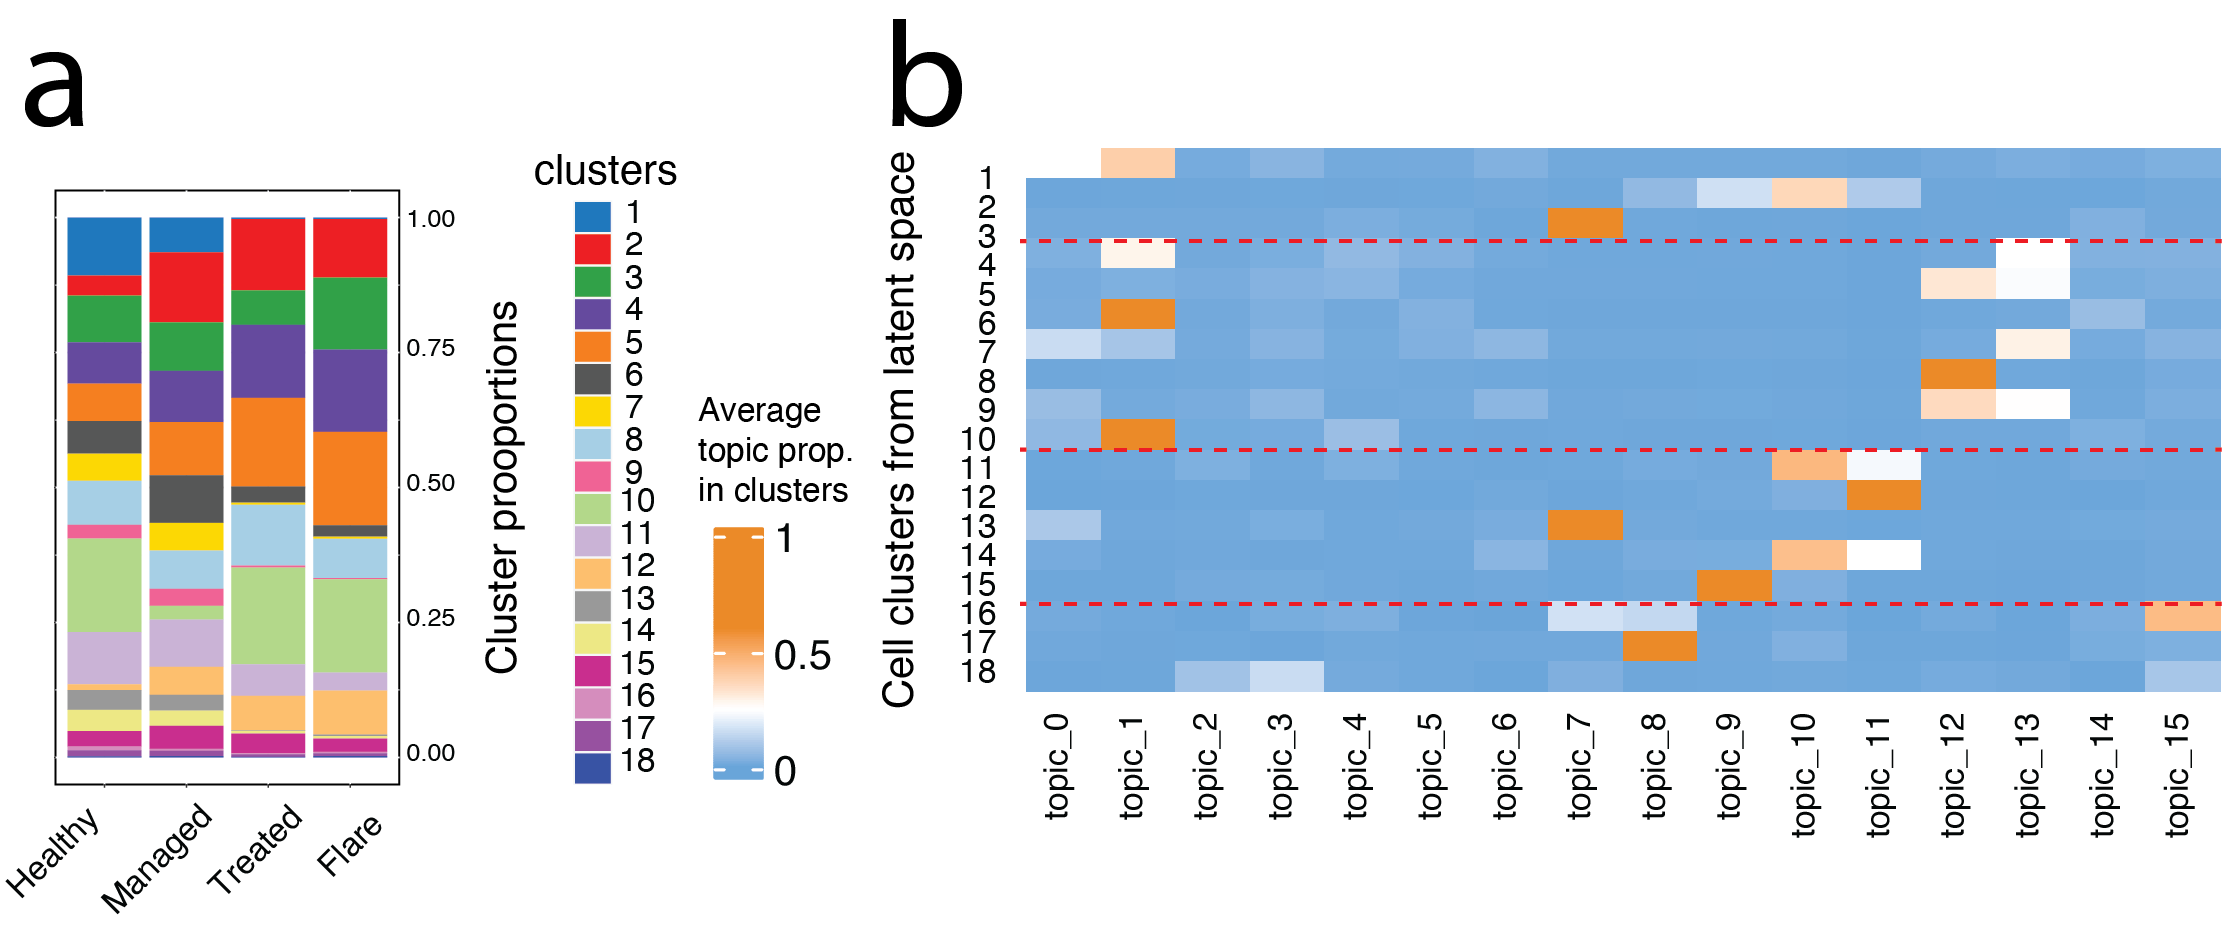
\includegraphics[width=\textwidth]{Figures/disease_strat_sftmx.png}
    \caption{\textbf{Cluster composition within samples is disease status dependent} a) Cell cluster proportion breakdown by SLE disease status shows cell composition within samples. b) Heatmap showing the median values of latent topic proportions across cells within each Louvain cluster. Clusters are shown along the rows of the heatmap.}
    \label{fig:diseasestrat}
\end{figure}

From the provided metadata of the scRNA-seq dataset in Perez \textit{et al.} \cite{sledata}, the trained model was analyzed in a disease-stratified fashion. Using the same Louvain clusters determined in the previous section (Fig.\ref{fig:cluster_umap}), differentially represented clusters were found depending on SLE disease status (Fig.\ref{fig:diseasestrat}a). Clusters 1, 6, 7, 9 and 11 capture primarily cells from healthy individuals or individuals with managed SLE. Cells in clusters 2 and 12 make up a significantly greater portion of cells from individuals with any level of SLE compared to healthy individuals. Some clusters make up a greater portion of cells from individuals with active disease phenotypes of SLE (treated vs. flare), such as clusters 4 and 5. Finally, cluster 10 appears in each condition except for individuals with managed SLE. The differences in cluster representation suggest that the cellular makeup of PBMCs is associated with disease status. 

To understand how each cluster relates to the estimated latent topic representation of cells, the average topic profile for cells in each cluster is constructed (Fig.\ref{fig:diseasestrat}b). From this, it is shown that many clusters that are differentially represented across disease conditions actually share many features, suggesting that cells in different clusters may correspond to the same general cell type, but have some minute differences in gene expression. For example, clusters 4 and 7 both have strong representations by topics 1 and 13 but cells in cluster 7 have a higher representation in topic 0. Cells in these clusters are shown to be most closely aligned with effector memory and regulatory CD4+ T cells (Fig.\ref{fig:cluster_ct}), yet are distinctly different in their latent topic profiles. 

\begin{figure}
    \centering
    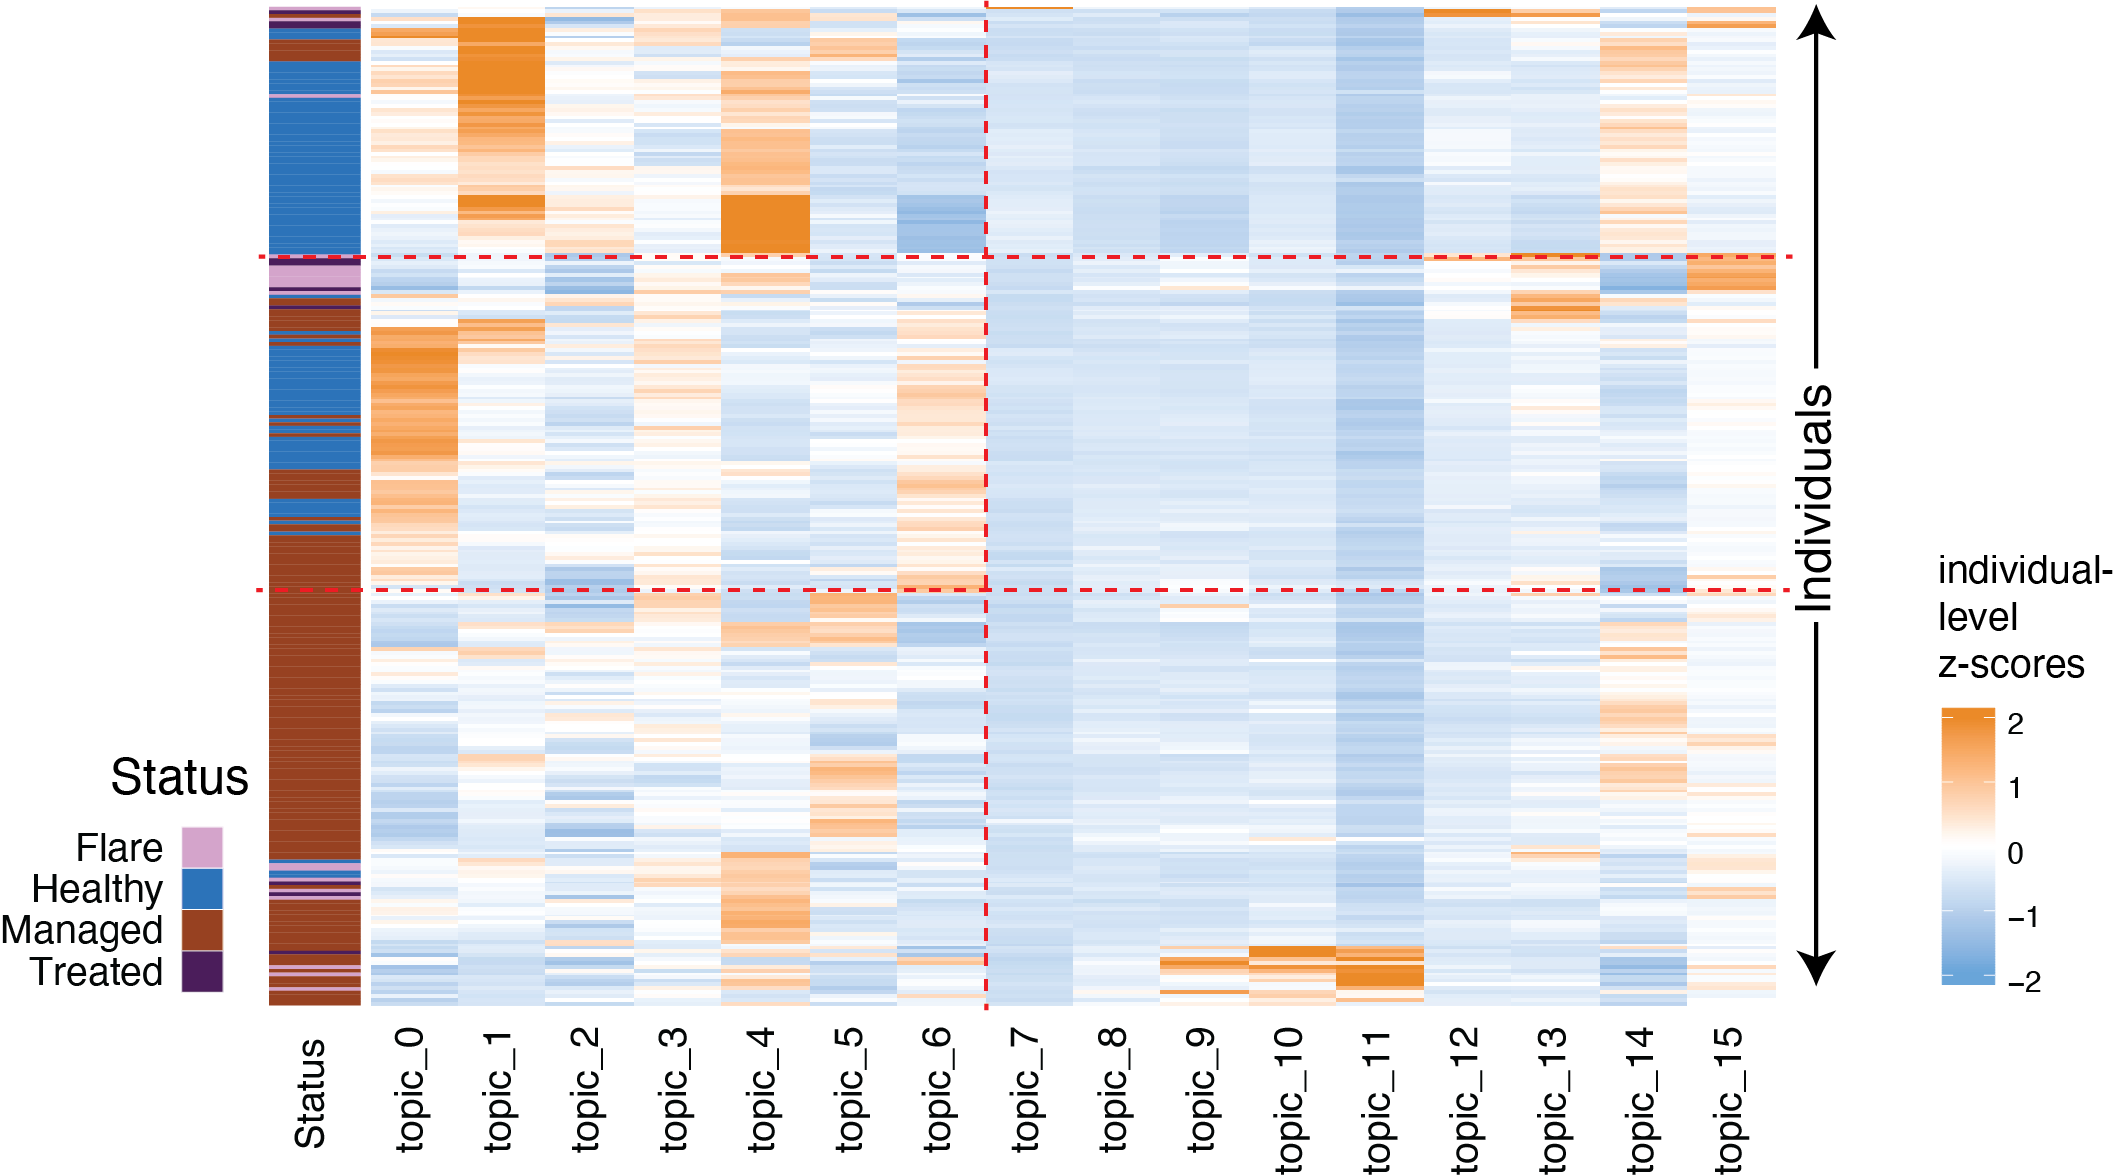
\includegraphics[width=\textwidth]{Figures/ind_median_latent_prof.png}
    \caption{\textbf{Individuals with identical disease status generally share latent topic patterns} Heatmap shows median latent topic profiles calculated for each individual included in the study. Rows represent each individual and are annotated by disease status.}
    \label{fig:ind_latent_prof}
\end{figure}

\begin{figure}
    \centering
    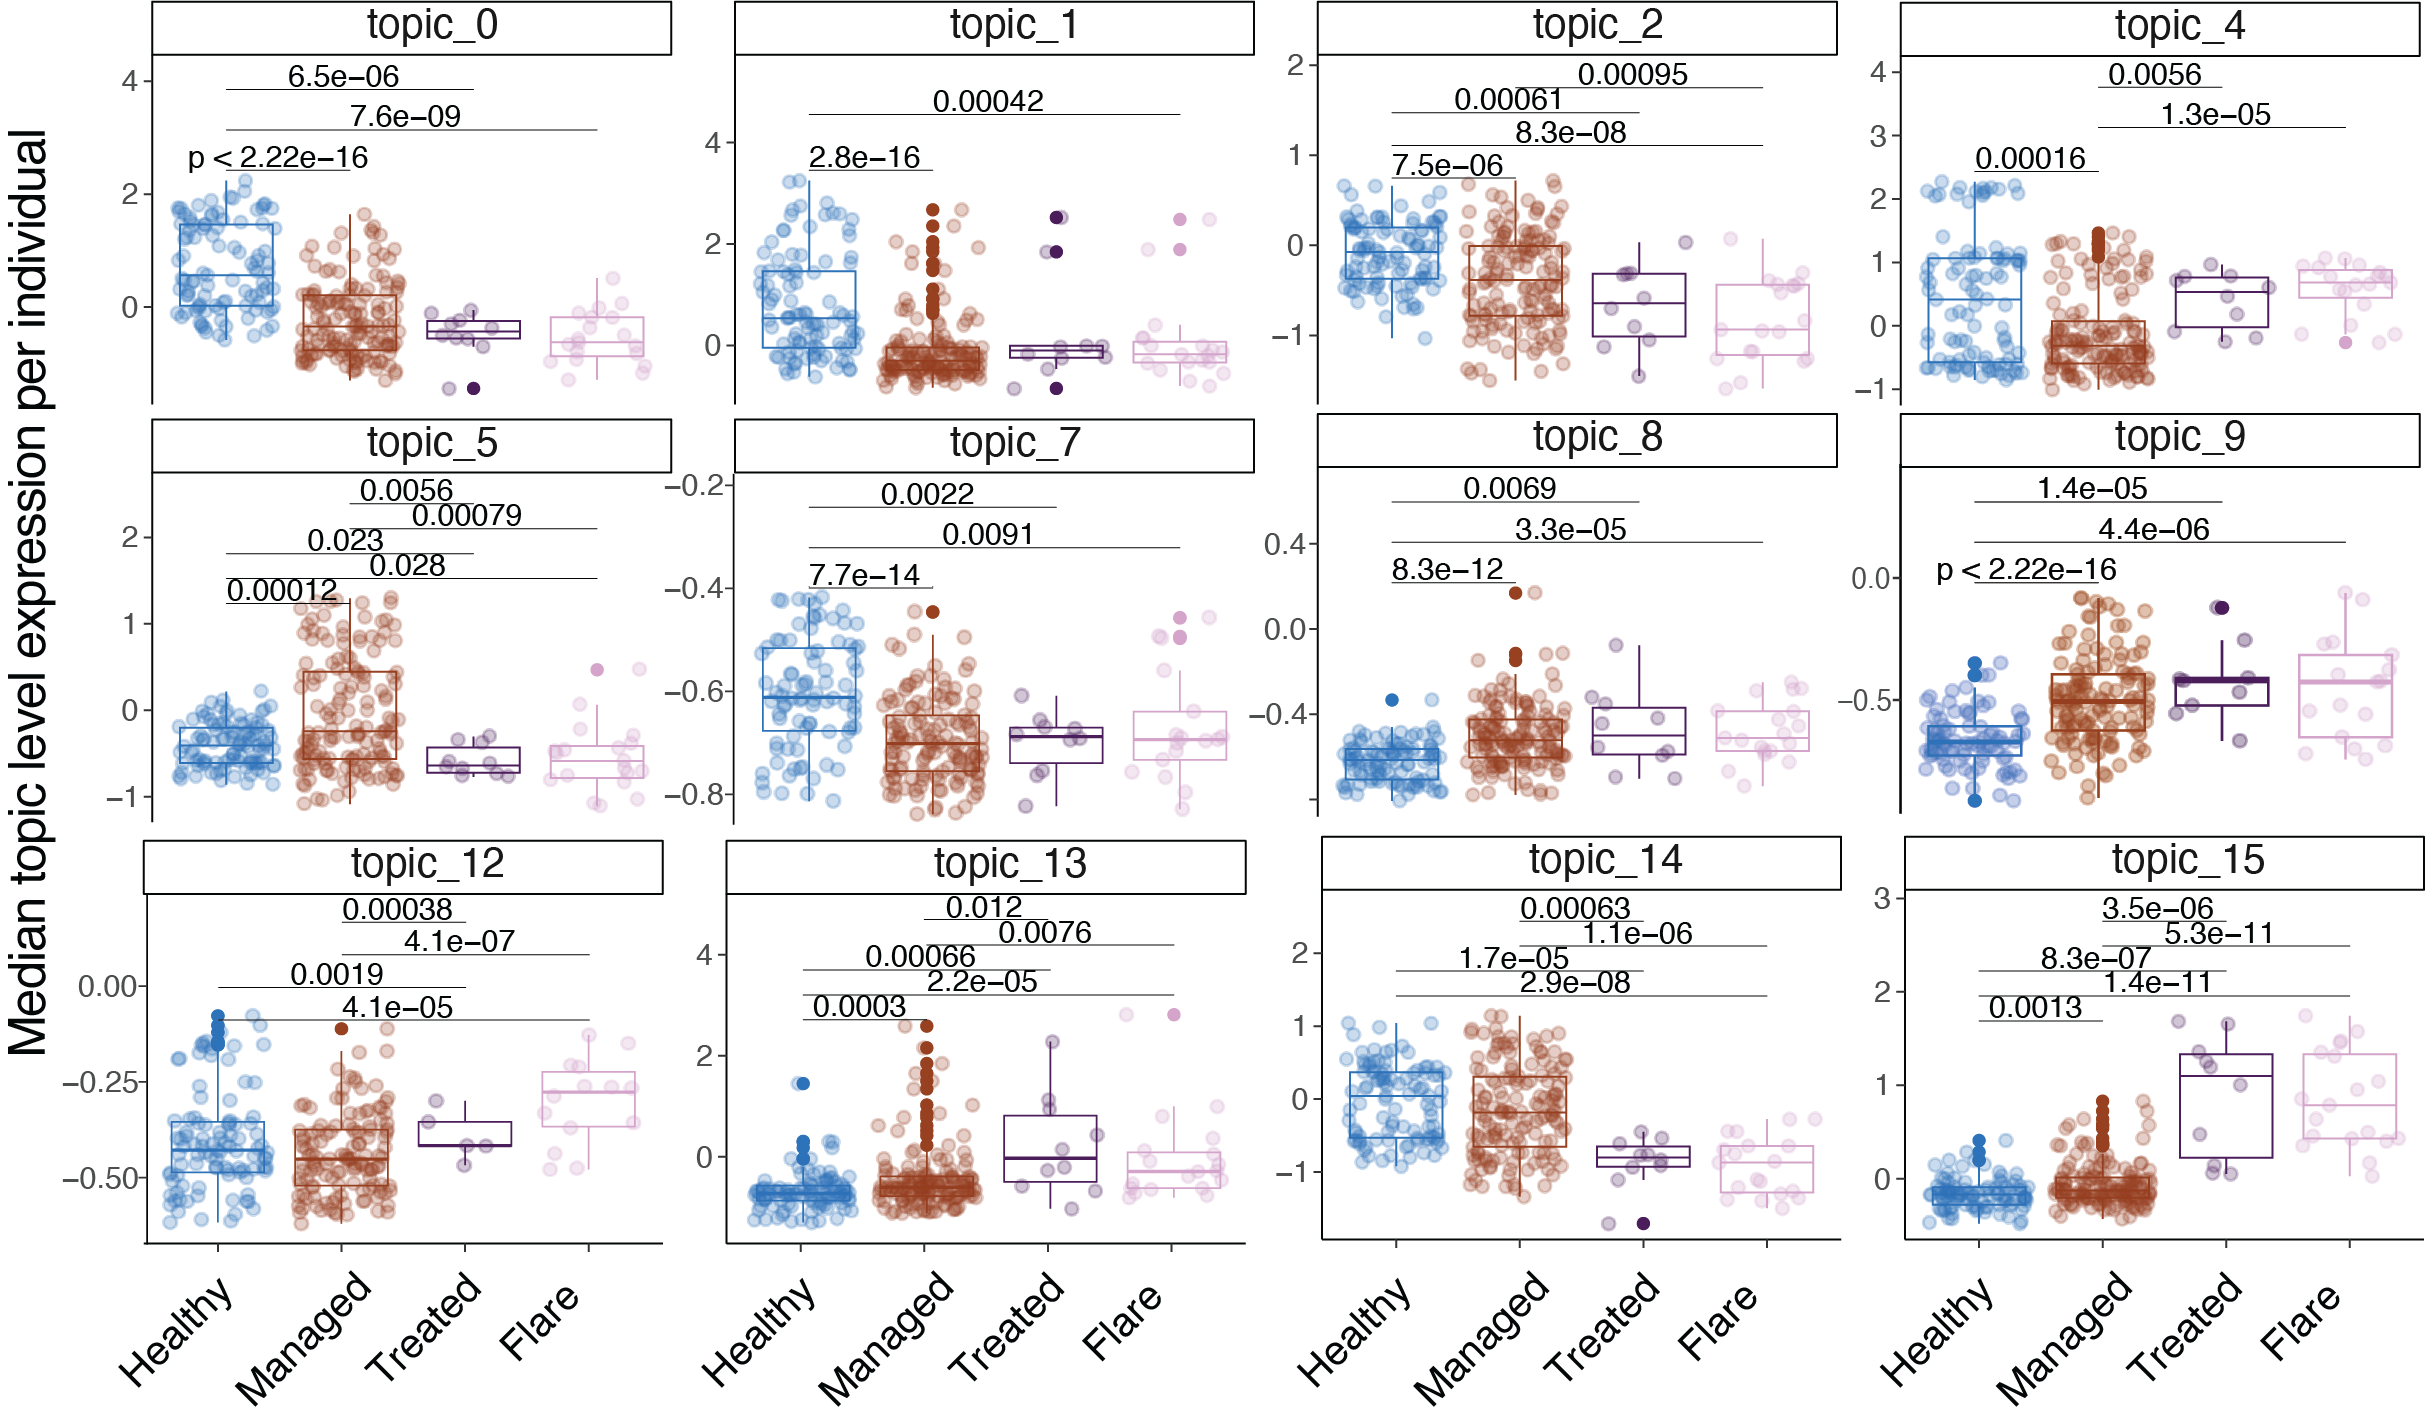
\includegraphics[width=\textwidth]{Figures/median_bxplt.png}
    \caption{\textbf{Disease status dependent differences exist in topic representation} Boxplots of median topic expressions per individual grouped by disease status. Topics with significant differences in median topic values between healthy and SLE individuals are shown. Significance between median expression values are calculated using Wilcoxon rank-sum tests between disease status individuals.}
    \label{fig:ind_bxplt}
\end{figure}

To better understand differences in topic representation as an effect of disease phenotype, the median topic profile for each individual included in the study is constructed (Fig.\ref{fig:ind_latent_prof}). From the latent profiles, a large variance in topic profiles across individuals is seen, yet individuals with similar profiles tend to share the same disease status. Wilcoxon rank-sum tests were performed on median latent topic values of individuals between disease status groups (Fig.\ref{fig:ind_bxplt}). Of note, topics 0 and 1 are  significantly differentially represented in healthy individuals compared to individuals with SLE of any status. Topic 0 separates cells found in cluster 7 from those in cluster 4, while topic 1 is seen in all clusters containing CD4+ T cells. Topic 12, which is represented in clusters corresponding to NK cells, CD8+ T cells and proliferating lymphocytes(Fig.\ref{fig:cluster_ct}, Fig.\ref{fig:diseasestrat}b), is significantly higher in individuals with treated and flare SLE conditions compared to healthy and managed SLE. Healthy individuals and those with managed SLE have a significantly higher level of topic 14 than those with an active SLE status, while the inverse is true for topic 15, suggesting a higher prevalence of intermediate immune cell states in individuals with active SLE while healthy and managed individuals have a higher prevalence of B cells and certain naive T lymphocytes (Fig.\ref{fig:cluster_ct}, Fig.\ref{fig:diseasestrat}b). Showing the differences in topic levels across disease statuses informs our investigation into the differentially regulated biological gene sets suggested by the latent-node level gene embeddings of the model. 

\newpage
\section{Functional Analysis of Latent Nodes}

\subsection{Node-level Gene Clustering}

\begin{figure}
    \centering
    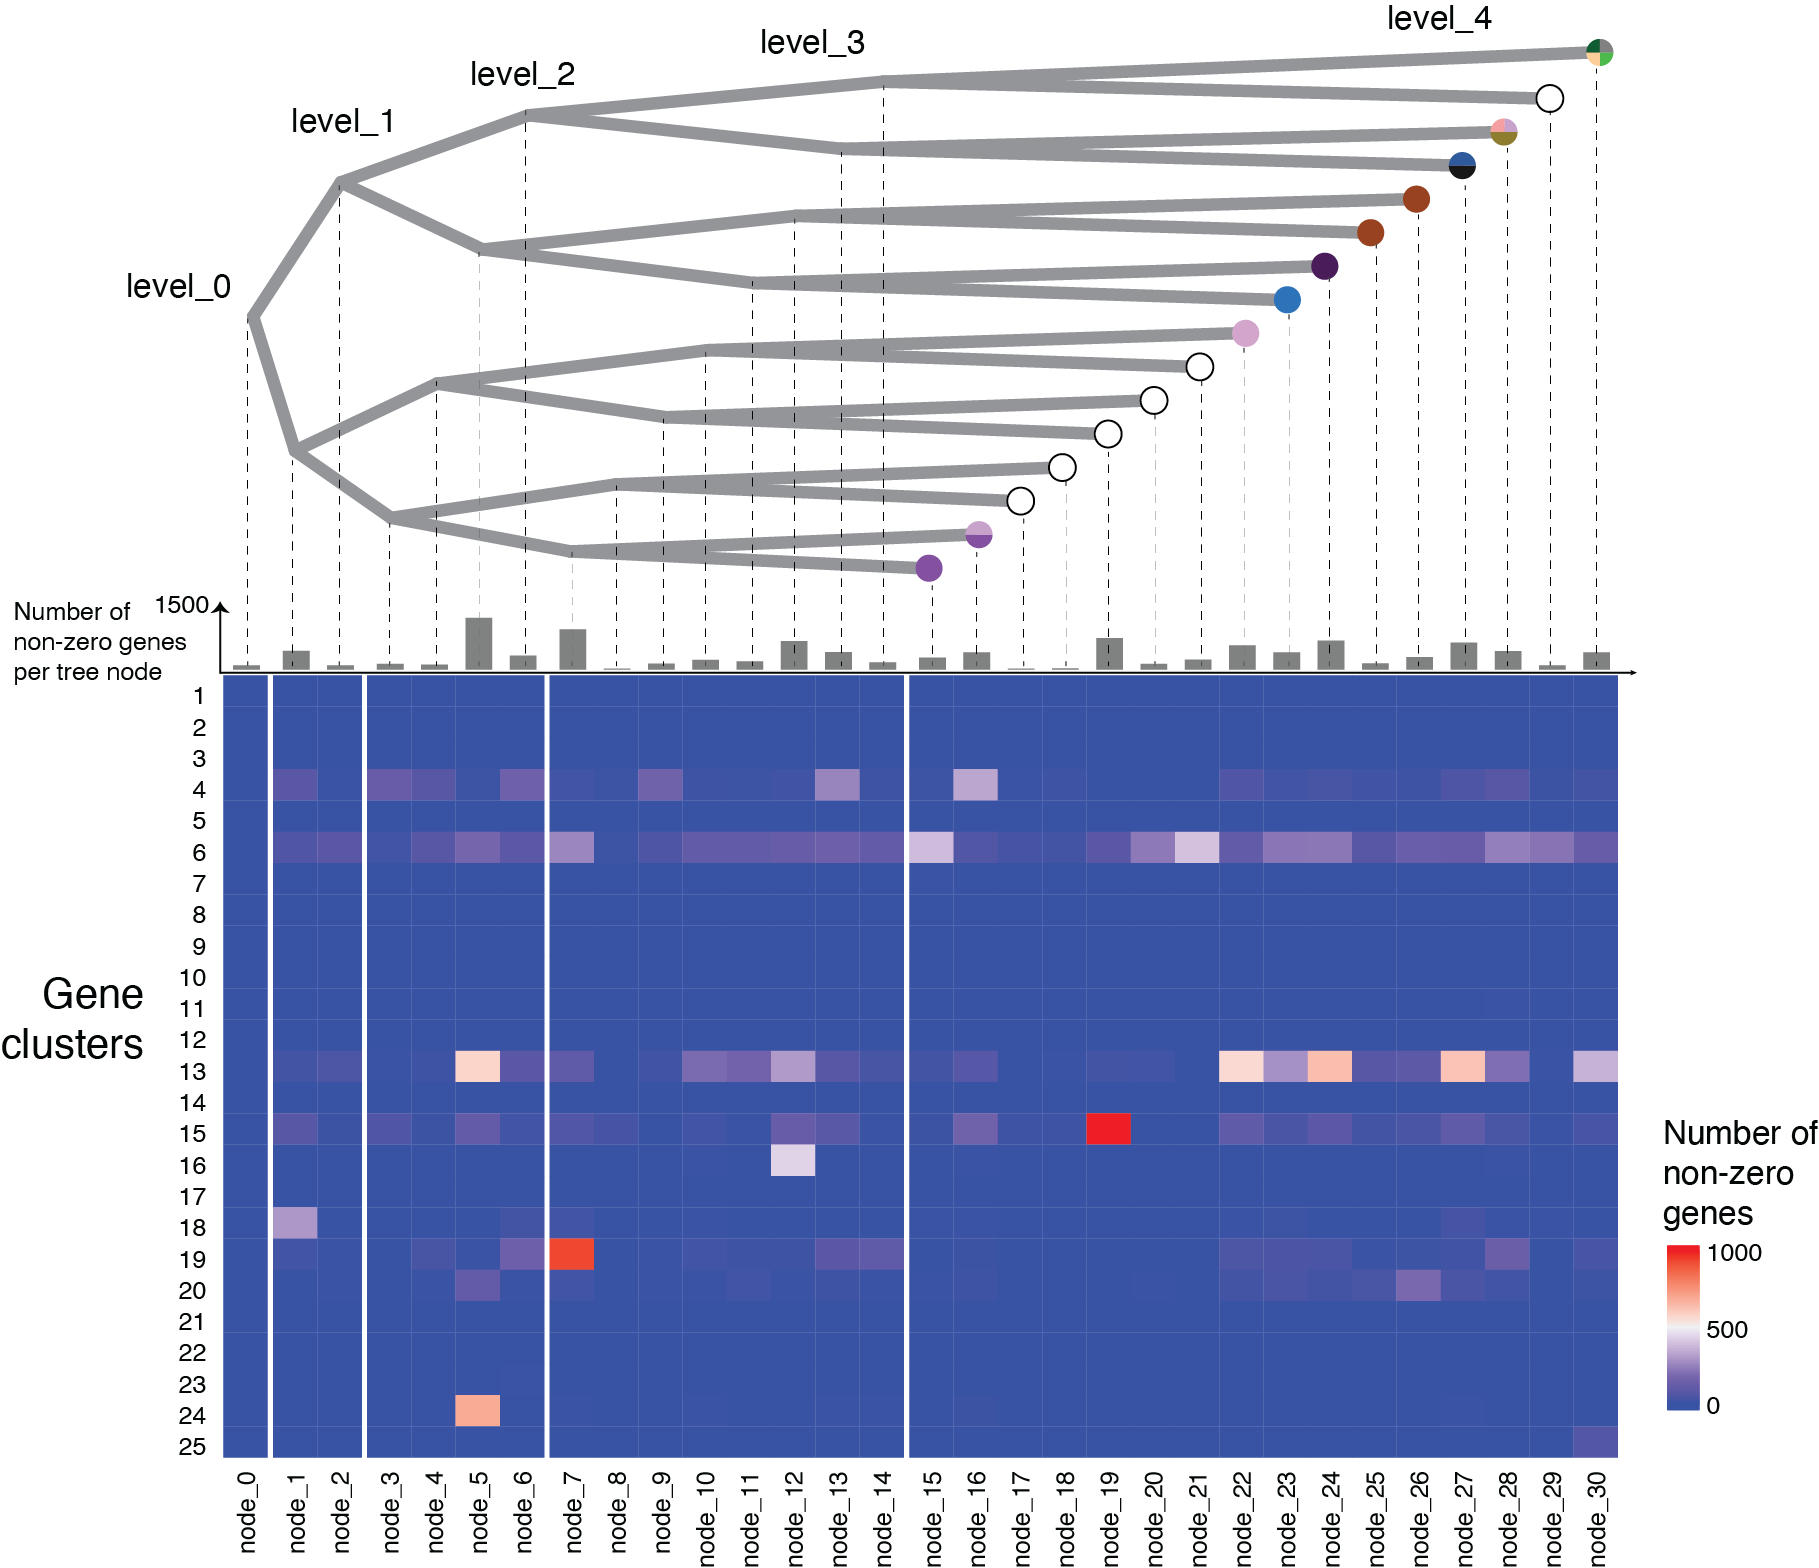
\includegraphics[width=\textwidth]{Figures/node_clusters.png}
    \caption{\textbf{Clustering of genes based on node-level embeddings show overarching gene programs} Heatmap shows number of significantly non-zero genes within each node that belong to gene clusters. Total numbers of non-zero genes per tree node are annotated above.}
    \label{fig:nodeanalysis}
\end{figure}

Further investigation was conducted on the number of genes that effectively define cell-type specific disease mechanisms using learned node-level gene vectors from LaRCH, namely $\hat{\beta}$ parameters before the tree-based topic-level aggregation. It is assumed that Bayesian variable selection prior can put zero values to unnecessary (or statistically weak) associations for irrelevant genes. Counting only the number of genes significantly deviating from zero, the number of genes needed for each tree node and level was counted (Fig. \ref{fig:nodeanalysis}). For brevity, genes were clustered into 25 distinctive gene modules by applying the Louvain clustering method on the 10-nearest neighbour gene-gene interaction graph (Fig.\ref{fig:nodeanalysis}). The Bayesian spike-and-slap prior ensured that the node-level gene programs are determined by a subset of genes between 50 to 1800 genes, with a median number of 429. Albeit, more genes were found on nodes 5 (cluster 24) and 7 (cluster 19), which correspond to T- and B-cell groups, respectively.

\subsection{Gene Set Enrichment Analysis of Node-Level Gene Embeddings}

\begin{figure}
    \centering
    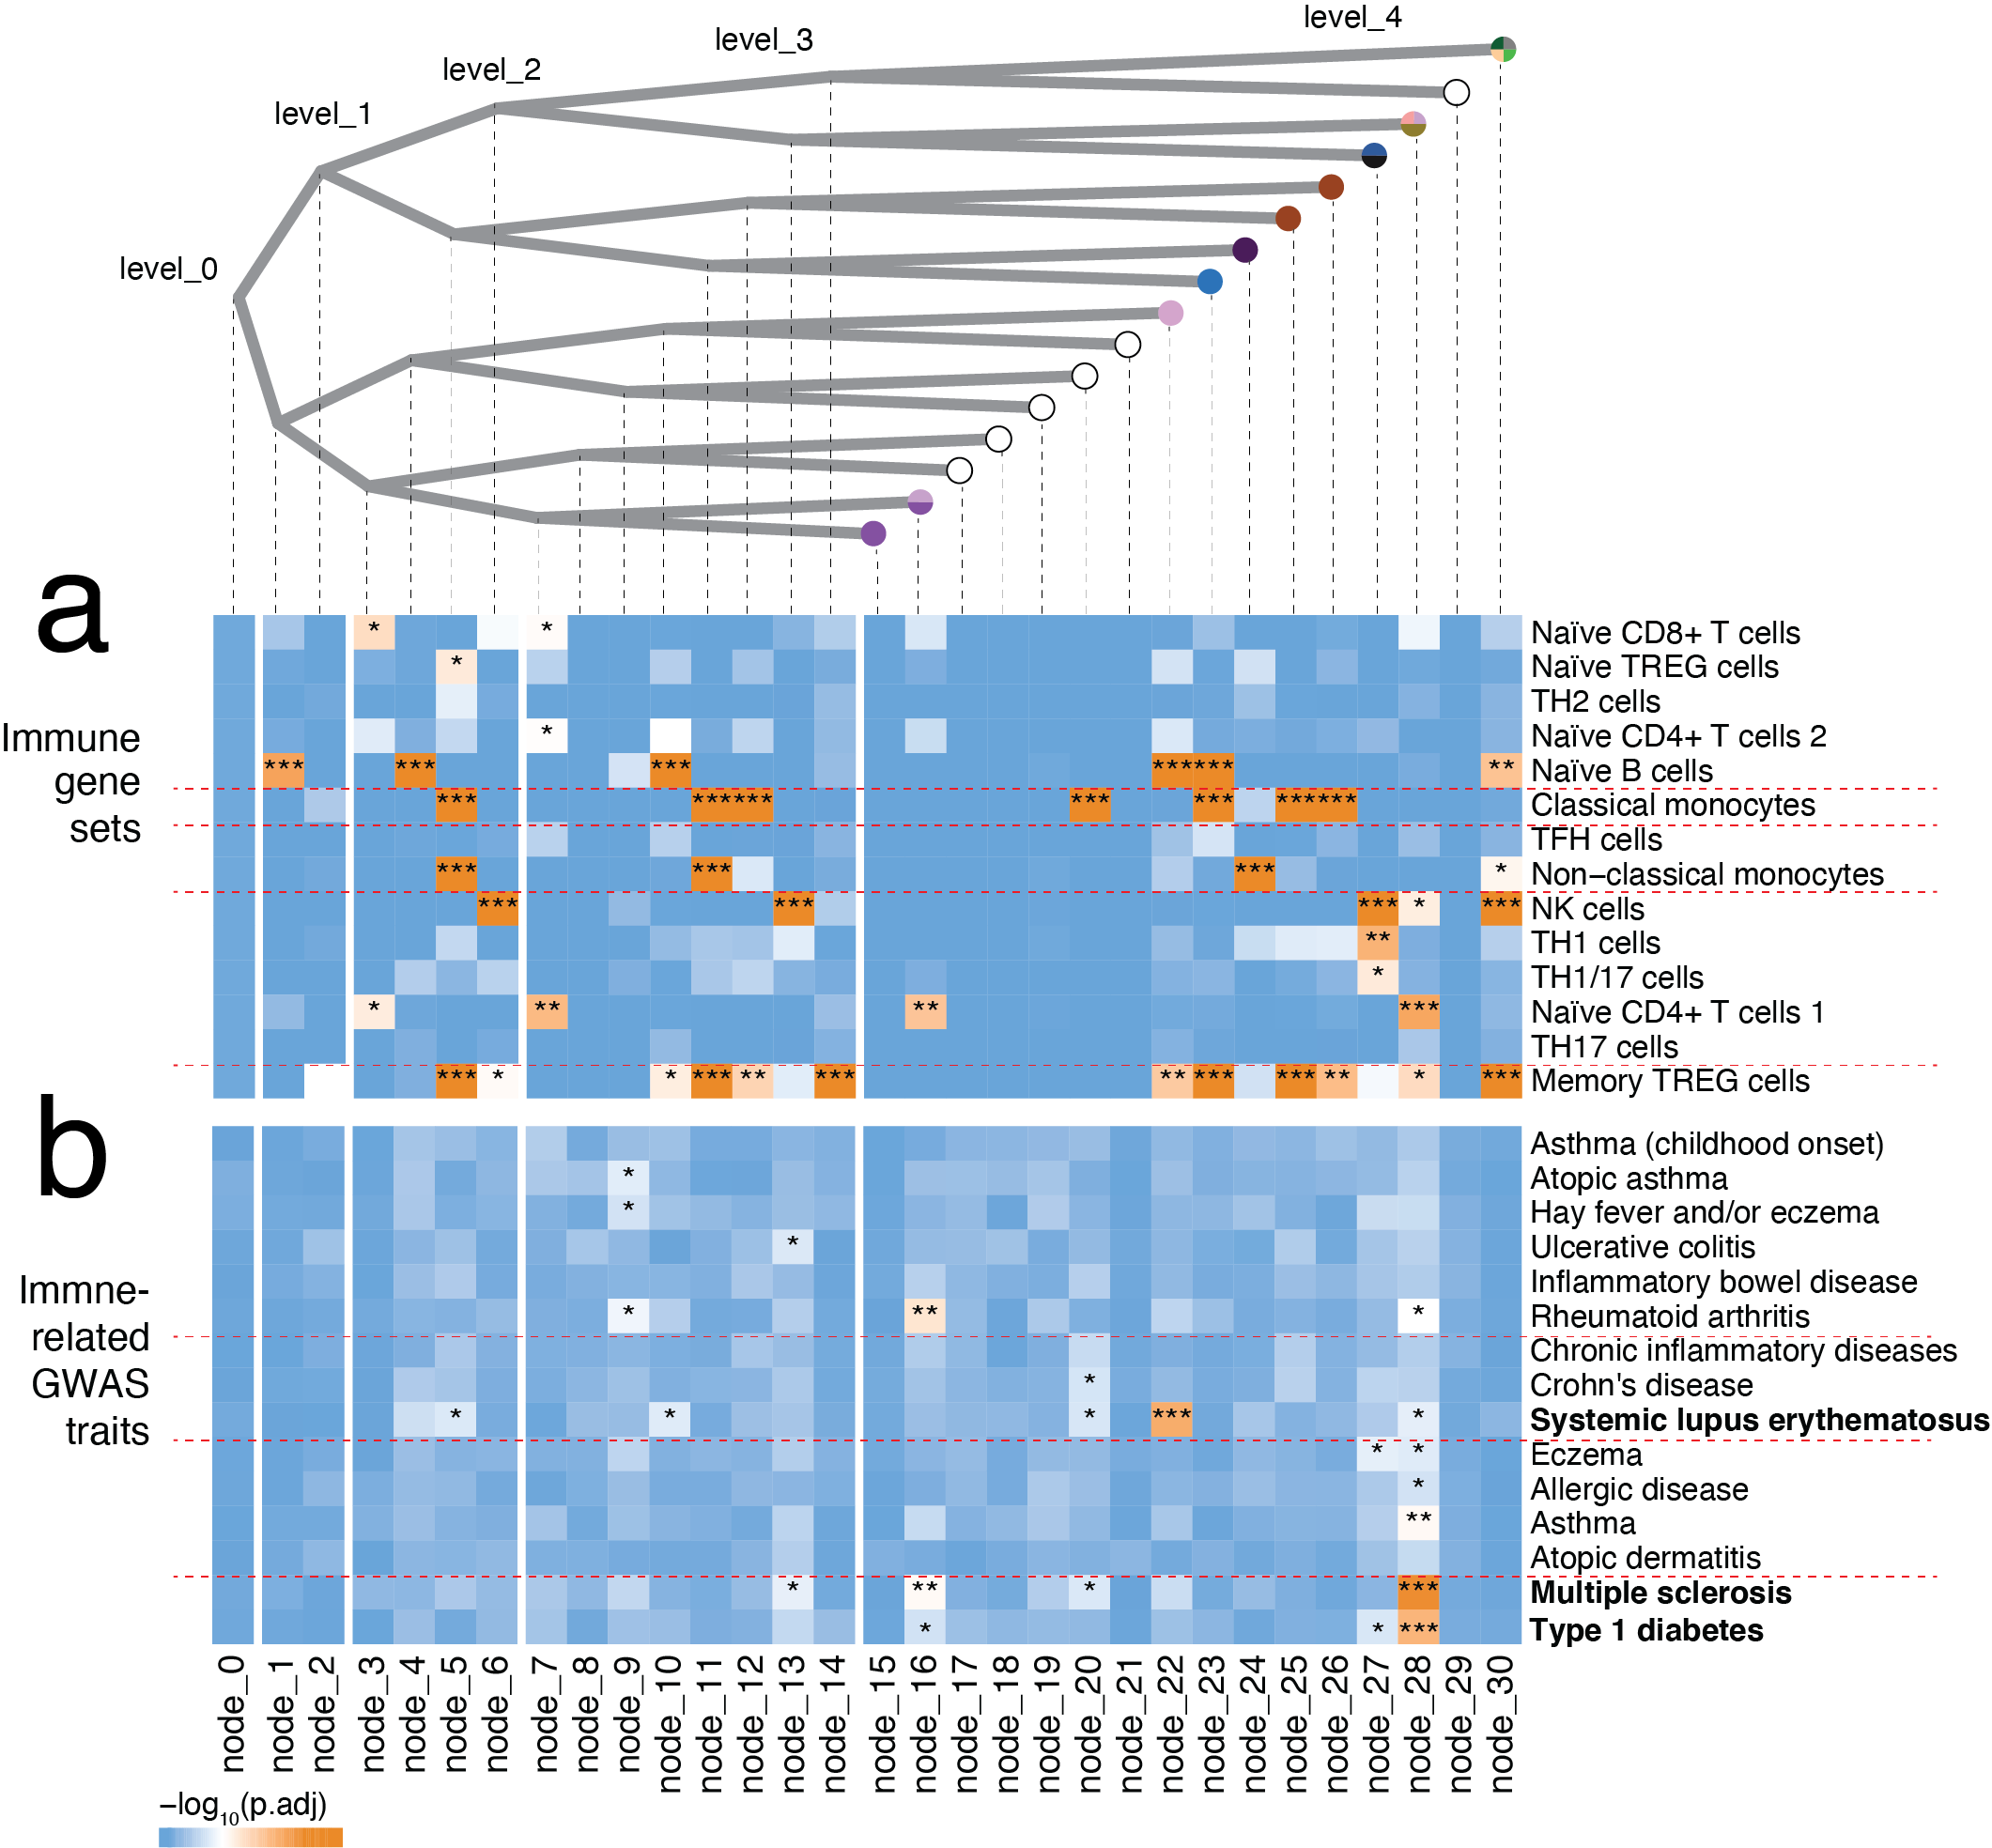
\includegraphics[width=\textwidth]{Figures/gsea.png}
    \caption{\textbf{Gene set enrichment analysis shows immune subset and disease relevant features described by latent node features} Heatmap shows the $-\log(p)$ enrichment significance of each gene set per node. Significance annotations are as follows: $*** - p < 0.0001, ** - p < 0.001, * - p < 0.01$.}
    \label{fig:gsea}
\end{figure}

Enrichment analysis of cell-type specific differentially expressed gene sets based on gene embedding values allows for further annotation of cell type relationships to latent topics. Ranked gene set enrichment analysis was performed using the \texttt{fgsea} R package \cite{fgsea} with the estimated embedding values $\hat{\beta}$ as the fgsea score. Gene sets used for enrichment analysis were obtained from the DICE database \cite{DICE1}, the NHGRI-EBI Catalog of human genome-wide association studies \cite{gwas_cat}, ImmuneSigDB \cite{godec2016compendium}, and the hallmark gene sets within MSigDB \cite{liberzon2015molecular}.

Gene sets related to immune function were found to be enriched in a number of relevant latnet nodes, suggesting functional phenotypic features represented through latent topic representation (Fig. \ref{fig:immune_gsea}). B cell-related genes are enriched at the early stages of the node tree, suggesting a distinct model lineage that these cells follow (Fig.\ref{fig:gsea}a). an enrichment of B cell-related genes in node 23 is also seen, along with classical monocyte and memory regulatory T cell-related genes. In Fig.\ref{fig:sle_tree}, topic 8 (made up of nodes 0, 2, 5, 11, and 23) was determined to correspond to dendritic cells, which canonically share lineage paths with both monocytes and lymphoid cells \cite{immunediff}. Topic 1 (made up of nodes 0, 1, 3, 7, and 16), which is significantly greater in healthy individuals (Fig.\ref{fig:ind_bxplt}), is enriched in genes relating to naive T cells, suggesting a loss of naive cells and concomitant increase in activated T cells in individuals with SLE. Gene sets of less prevalent sub-types, such as Th17 and Th2 helper T cell subsets, are not found to be significantly enriched in any node as they are difficult to distinguish amidst a heterogeneous sample. 

Enrichment analysis of GWAS (GWAS) gene sets pertaining to immunological disease reveals node-level differences in disease manifestation (Fig.\ref{fig:gsea}b). Disease-relevant gene sets are mainly found to be enriched in nodes at deeper levels of the tree, suggesting that disease manifestations are cell-type specific, rather than common features across many cells. GWAS genes relating to SLE are enriched primarily in node 22, which corresponds to topic 7. This node also is related to B cell function (Fig.\ref{fig:nodeanalysis}b), which is in line with the fact that SLE is often characterized by abnormal autoreactive B cells \cite{slebcells}. Node 28, corresponding to topic 13, is enriched in gene sets relating to other autoimmune diseases, such as multiple sclerosis and type-1 diabetes, as well as memory Treg cells, naive CD4+ T cells, and NK cells. Autoreactive T cell function is the primary driver of these diseases \cite{ms, t1d} and the corresponding topic 13 is enriched in individuals with SLE (Fig.\ref{fig:ind_bxplt}), suggesting an additional role of autoreactive T cells in SLE pathogenesis. 

\newpage
\section{Node-level Marker Genes}

Node-level gene embedding values allow for the identification of significant marker genes that contribute to the gene expression signature of cells represented by specific latent topics. From the node-level marker genes, biological meaning can be extracted to provide insight on cell-type specific features associated with SLE.

\subsection{Marker Gene Significance Testing}

Significant marker genes for each latent node were obtained using  parameters learned in the decoder component of LaRCH. $\hat{\beta}$ and $\mathbb{V}[\hat{\beta}]$, calculated using (\ref{eq:betahat_est}) and (\ref{eq:betahat_var}), were fed directly into the \texttt{ashr} R package described in the Stephens \textit{et al.} \cite{ashr}. This package uses an emprical Bayes approach for large-scale hypothesis testing and false discovery rate estimation. Significant genes are selected as those with \texttt{qvalue} $< 0.05$. The number of significant genes per node is detailed in table \ref{tab:sig_genes}. Unique significant genes are used to identify gene features that separate a specific latent tree node from its parent and sibling nodes, therefore playing a role in driving the differentiation from one topic path to another. A significant gene is considered unique to a node if it does not also appear as a significant gene it its parent a direct sibling node. These gene counts are summarized in table \ref{tab:unique_sig_genes}.

\subsection{Marker Genes of Interest}
\begin{figure}
    \centering
    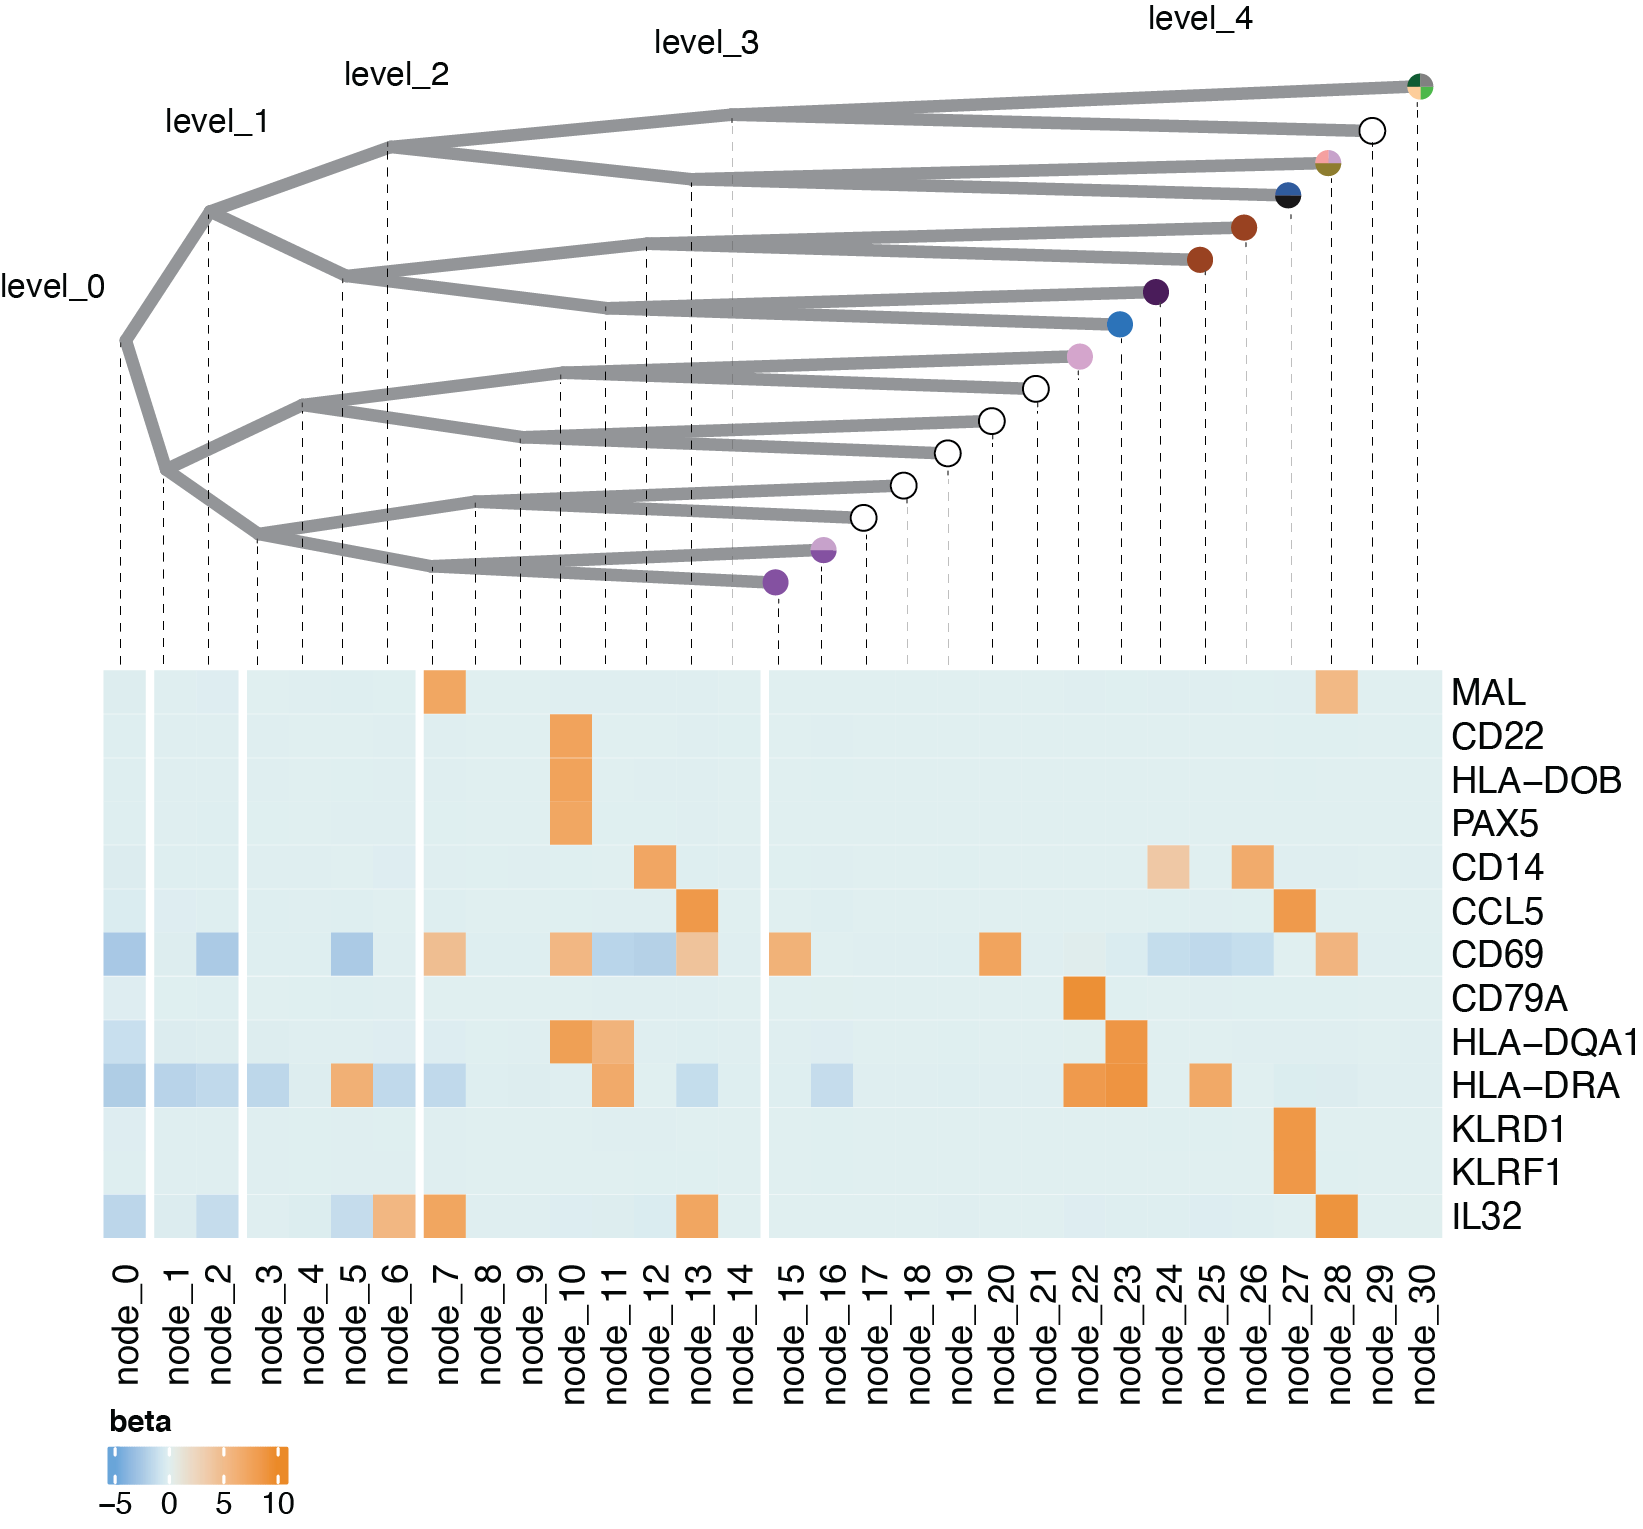
\includegraphics[width=\textwidth]{Figures/markers.png}
    \caption{\textbf{Canonical immune subset markers are captured in latent tree nodes of the topic model} Heatmap shows estimated node-wise gene embedding values $\hat{\beta}$ of genes previously identified as marker gene for immune cell subsets.}
    \label{fig:marker_genes}
\end{figure}

From the list of significant genes for each tree node, the top ten genes with the greatest absolute $\hat{\beta}$ value from each node are selected for further investigation. The top 80 genes from this list are shown in figure \ref{fig:top_beta_hm}.

\subsubsection{Significant Node-level Immune Marker Genes}
Within this list are several known immune cell type markers (Fig. \ref{fig:marker_genes}). 

MAL is a protein coding gene that is selectively expressed during T cell differentiation \cite{alonso1987cdna}. It is seen in  nodes 7 and 28, which correspond to topics 0, 1, and 13. This is in accordance with the labeling of these topics as representing T cell subsets in figure \ref{fig:sle_tree}. CD69 is a membrane-bound type II C-lectin receptor and is a marker of lymphocyte activation \cite{cibrian2017cd69}. It is identified as a marker gene in a number of nodes, all which correspond to topics containing lymphocyte subsets (0, 1, 7, 12, 13). Interestingly, this gene is also down regulated in nodes associated with monocyte subsets.

NK cells are identified by KLRD1 and KLRF1, two killer cell lectin like receptors which are markers of node 27, the leaf node of topic 12 \cite{cozar2021tumor}.

In nodes corresponding to topic 7, which is almost exclusively present in B cells, a number of B cell markers are present. In node 10 and 22, the two final nodes in the path of topic 7, CD22, HLA-DOB, PAX5, and CD79a are uniquely expressed in B cells. \cite{moyron2002expression, nagarajan2002class, chu2001cd79, desouki2010pax} HLA-DRA is identified as a marker gene in node 22 along with a number of other tree nodes that correspond with topics 8-11 which are associated with dendritic cells and monocytes. HLA-DRA is a HLA class II molecule that is a component of the major histocompatibility complex (MHC) II and is expressed on the surface of various antigen presenting cells (APCs) including B lymphocytes, dendritic cells, and monocytes \cite{VANDENELSEN200467}. CD14, a well known marker of monocyte \cite{goyert1986biochemistry}, is a top gene in nodes 12, 24, and 26 which correspond to topics 9, 10, and 11, topics associated with monocytes. 

From the analysis in this chapter, node-level immune cell markers are congruent with cell type assignments presented in Perez \textit{et al.} \cite{sledata}. The presentation of immune cell type marker genes as significant genes in tree nodes demonstrates the ability for the LaRCH model results to inform cell type assignments to scRNA-seq datasets using their latent topic representations. 

\subsubsection{Significant Node-level Genes with Potential SLE Disease Association}
\label{cha:genes}
\begin{figure}
    \centering
    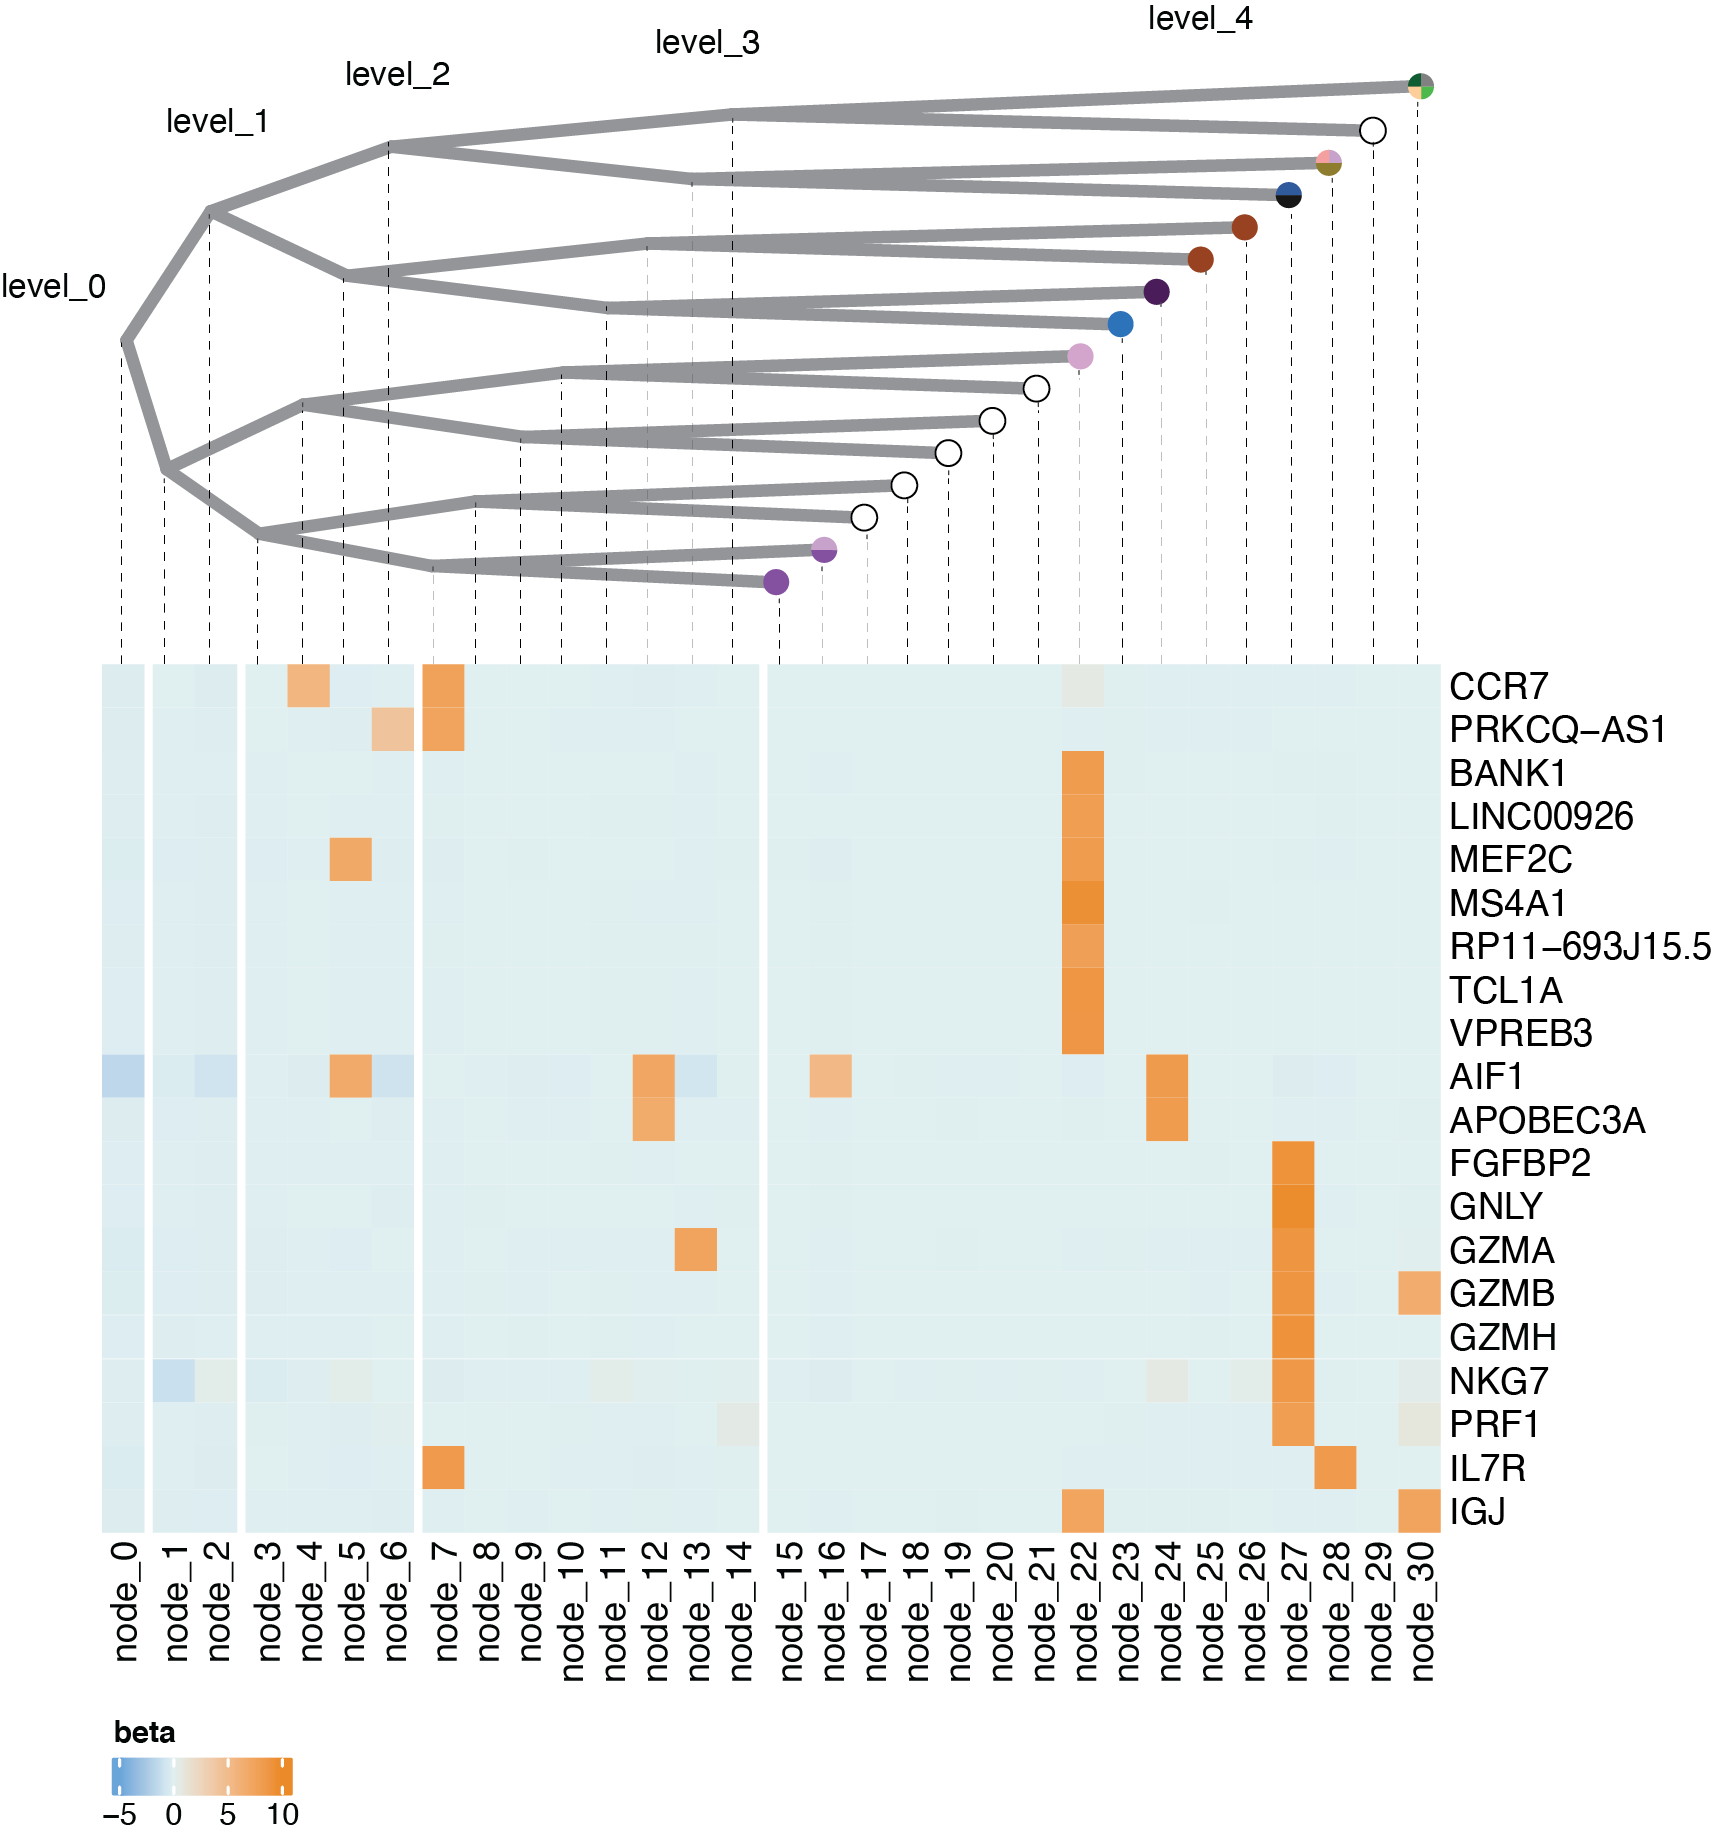
\includegraphics[width=\textwidth]{Figures/immune_genes.png}
    \caption{\textbf{Node-level gene embeddings reveal potential genes of interest with regards to SLE pathogenesis} Heatmap shows estimated node-wise gene embedding values $\hat{\beta}$ of genes with relevant immune function to SLE disease mechanisms.}
    \label{fig:immune_genes}
\end{figure}

Analysis of significant genes outside of canonical immune subset markers paired with the SLE disease status dependent differential topic representation provides insight into potential cell-type specific mechanisms associated with disease phenotypes. 

Patients experiencing SLE flares show significantly elevated representation of topic 12 \ref{fig:ind_bxplt}. This topic is associated with CD8+ T lymphocytes and nodes in this topic contain GZMH, GZMB, and PRF1 as marker genes. It has been shown that patients with SLE show elevated levels of GZMH+ cytotoxic CD8+ T cells \cite{sledata}. Similarly, PRF1 and GZMB expressing CD8+ T cells have been correlated with SLE disease activity \cite{blanco2005increase}. 

Topic 7, which contains node 22, has a significantly lower representation in patients with SLE. Node 22 has a number of significant genes associated with B cell function, including BANK1. BANK1 encodes a scaffolding protein expressed predominantly in B cells. Variants in this gene have been shown to elevate risk of SLE by increasing susceptibility to autoantibodies \cite{dam2016bank1}.

Patients with SLE show elevated representation in topic 9. The corresponding nodes of this topic, nodes 12 and 24 contain AIF1 and APOBEC3A as significant genes. AIF1 has been shown to be linked with the activation of macrophages and is implicated in several inflammatory diseases \cite{de2023aif1}, making it a viable candidate for exploration of macrophage related mechanisms driving SLE. APOBEC3A is a part of the APOBEC3 family of cytidine deaminase. APOBEC3A gene expression is induced by type I interferon (IFN-I) response during viral infections and plays an important role in defence against viral infection \cite{taura2022apobec3a}. Patients with SLE have been shown to have elevated expression of APOBEC3A compared to healthy controls, especially in those with flares \cite{perez2021sustained} and there is justification for further exploration into the role it plays in autoimmune disease \cite{liu2023underexplored}.

Topics 0 and 1 latent values are significantly higher in healthy individuals than patients with SLE \ref{fig:ind_bxplt}. A shared node in the paths of these topics is node 7 which contains the marker genes CCR7 and PRKCQ-AS1. CCR7 is a chemokine receptor that is critical to the function of naïve T cells \cite{britschgi2008dynamic}. This suggests an expected reduction of naïve CD4+ T cells in patients with SLE. PRKCQ-AS1 is a long non-coding RNA (lncRNA) that has recently been associated with the regulation of the expression of IL-1$\beta$, IL-6, and IL-8 in fibroblasts with TNF-$\alpha$ stimulation \cite{zhao2023role}, as well as the regulation of glycolysis and mitochondrial functions in thyroid carcinoma \cite{zhang2023fasting}. SNPs in this gene have also been associated with asthma, eczema, and allergic rhinitis \cite{shi2023characterization}, making it a viable candidate for exploration in the context of CD4+ T cell driven SLE manifestation. 




